\chapter{Odporna optymalizacja}\label{ch:minmax}
\thispagestyle{chapterBeginStyle}





W poprzednim rozdziale zapoznaliśmy się z~podstawowymi informacjami na temat problemu odnajdywania minimalnych drzew rozpinających w~grafach oraz poznaliśmy sposoby radzenia sobie z~nim.
Do tej pory jednak nie poruszyliśmy najistotniejszego dla nas tematu: \textbf{optymalizacji odpornej} na czynniki zewnętrzne.
Co przez to należy rozumieć?
Do tej pory poznaliśmy algorytmy, które potrafią rozwiązywać problem w~środowisku zamkniętym --- idealnym, w~którym nic nie ma prawa się zmieniać przez cały czas pracy algorytmu.
W~tym rozdziale omówimy modele problemów nie posiadających takiego ograniczenia --- w~modelach tych dane nie tylko będą mogły się zmieniać, ale będziemy także dopuszczać możliwość bycia nieświadomym tych zmian.
W~charakterze podsumowania, formalnie zapiszemy model jednego z~wariantów przedstawionych problemów, wskazując tym samym ogólne podejście do jego rozwiązania.




\section{Scenariusze dyskretne a~ciągłe}




W poprzednim rozdziale skupialiśmy swoją uwagę na problemie wyszukiwania minimalnego drzewa rozpinającego w~grafie $G = \left( V, E \right)$, czyli takiego zbioru krawędzi $T^{\ast}$, który łączył ze sobą wszystkie wierzchołki w~grafie, a~jednocześnie którego suma kosztów krawędzi $e \in T^{\ast}$ była możliwie najmniejsza.
Formalnie:

\begin{equation}
	T^{\ast}_{G = \left( V, E \right)} = \left\{ e \in E \; : \; T^{\ast}_{G = \left( V, E \right)} \in \mathcal{T}_{G} \; \wedge \; \left( \forall T^{\prime} \in \mathcal{T}_{G} \right) \; \sum_{ \mathclap{e \in T^{\prime} }} c_{e} \geqslant c_{ T^{\ast}_{ G = \left( V, E \right) } } \right\}\text{,}
\end{equation}
gdzie $\mathcal{T}_{G}$ oznaczał zbiór wszystkich drzew możliwych do skonstruowania w~grafie $G$, $c_{e}$ --- koszt krawędzi $e \in E$, zaś $\sum_{ e \in T^{\prime} } c_{e} = c_{T^{\prime}}$ --- sumę kosztów wszystkich krawędzi, która wynika ze \textbf{scenariusza}.
Scenariuszem $\textbf{s}$ zatem nazwiemy zbiór definiujący koszt dla każdej krawędzi w~grafie: $\textbf{s} = \left\{ c^{\textbf{s}}_{e_{i}} : i \in \left\{ 1, \dots, \left| E \right| \right\} \right\}$.
Na rysunku \ref{fig:scenarioExample} odpowiednio widzimy przykłady trzech różnych scenariuszy, zastosowanych do tego samego drzewa.
Rzecz jasna, zależnie od kosztów jakie zostaną narzucone krawędziom przez dany scenariusz, zwracane przez dotychczas poznane algorytmy rozwiązania będą się różnić.
Zwróćmy uwagę na rysunek \ref{fig:scenarioExample:b}, gdzie celowo nie zostały ujawnione koszty scenariusza --- jedyne co o~nim wiemy to to, że żaden koszt krawędzi w~tym scenariuszu nie jest mniejszy od kosztu odpowiadającej mu krawędzi w~$\textbf{s}_{1}$, ani większy od kosztu tej samej krawędzi w~scenariuszu $\textbf{s}_{3}$.
Taki rodzaj scenariusza nazywamy \textbf{scenariuszem ciągłym}, zaś scenariusze, których poszczególne koszty krawędzi są najmniejsze (bądź największe) spośród wszystkich scenariuszy, nazywamy \textbf{scenariuszami granicznymi/krytycznymi} (odpowiednio \textbf{scenariuszem najlepszego/najgorszego przypadku}).

\begin{figure}[!htbp]
	\null\hfill
	\begin{subfigure}[b]{0.32\textwidth}
		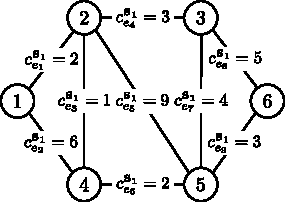
\includegraphics[width=\textwidth]{Chapter_II/SCENARIO-example/a}
		\caption{}
		\label{fig:scenarioExample:a}
	\end{subfigure}
	\hfill
	\begin{subfigure}[b]{0.32\textwidth}
		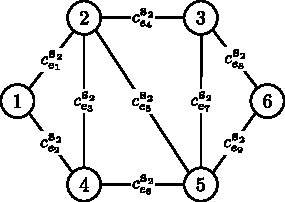
\includegraphics[width=\textwidth]{Chapter_II/SCENARIO-example/b}
		\caption{}
		\label{fig:scenarioExample:b}
	\end{subfigure}
	\hfill
	\begin{subfigure}[b]{0.32\textwidth}
		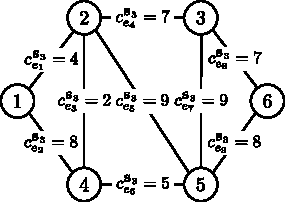
\includegraphics[width=\textwidth]{Chapter_II/SCENARIO-example/c}
		\caption{}
		\label{fig:scenarioExample:c}
	\end{subfigure}
	\hfill\null
	\caption{
		Scenariusze $\textbf{s}_{1}$, $\textbf{s}_{2}$, $\textbf{s}_{3}$ dla grafu nieskierowanego $G = \left( V, E \right)$, $V = \left\{ 1, 2, \dots, 6 \right\}$, $E = \left\{ e_{i} : i \in \left\{ 1, \dots, 9 \right\} \right\}$.
		\textbf{(a)}~Scenariusz najlepszego przypadku $\textbf{s}_{1} = \left[ 2, 6, 1, 3, 9, 2, 4, 5, 3 \right]$.
		Dla scenariusza zachodzi: $\left( \forall i \in \left\{ 1, \dots, 9 \right\} \right) c^{\textbf{s}_{1}}_{e_{i}} \leqslant c^{\textbf{s}_{2}}_{e_{i}}$.
		Scenariusz o~takich właściwościach będziemy też oznaczać jako $\underline{\textbf{s}}$.
		\textbf{(b)}~Scenariusz ciągły $\textbf{s}_{2}$.
		Koszty tego scenariusza zdefiniowane są następująco: $\left( \forall i \in \left\{ 1, \dots, 9 \right\} \right) c^{\underline{\textbf{s}}}_{e_{i}} \leqslant c^{\textbf{s}_{2}}_{e_{i}} \leqslant c^{\overline{\textbf{s}}}_{e_{i}}$.
		\textbf{(c)}~Krytyczny scenariusz najgorszego przypadku $\textbf{s}_{3} = \left[ 4, 8, 2, 7, 9, 5, 9, 7, 8 \right]$.
		Dla scenariusza zachodzi: $\left( \forall i \in \left\{ 1, \dots, 9 \right\} \right) c^{\textbf{s}_{2}}_{e_{i}} \leqslant c^{\textbf{s}_{3}}_{e_{i}}$.
		Scenariusz o~takich właściwościach będziemy też oznaczać jako $\overline{\textbf{s}}$.
	}
	\label{fig:scenarioExample}
\end{figure}

Przedstawione rodzaje scenariuszy można rozważać dla wszystkich problemów odpornej optymalizacji dyskretnej jakie tutaj wymienimy.
W~przypadku problemu minimalizacyjnego, jakim jest omawiany przez nas problem znajdowania minimalnego drzewa rozpinającego, krytyczne scenariusze najlepszego i~najgorszego przypadku będziemy oznaczać odpowiednio przez $\underline{\textbf{s}}$ oraz $\overline{\textbf{s}}$, gdzie $0 \leqslant \underline{\textbf{s}} \leqslant \overline{\textbf{s}}$.
Dla problemów maksymalizacyjnych znaczenie przedstawionych symboli byłoby zgoła odwrotne: $\overline{\textbf{s}}$ oznaczałby krytyczny scenariusz o~największych współczynnikach (najlepszego przypadku), zaś $\underline{\textbf{s}}$ --- najgorszego, gdzie każdy jego współczynnik nie byłby większy od dowolnego z~odpowiadających mu współczynników w~pozostałych scenariuszach.
\textbf{Scenariuszem dyskretnym} (ang. \textit{discrete scenario}) będziemy natomiast nazywać każdy scenariusz, który ma zdefiniowane koszty dla każdej krawędzi.
Takimi scenariuszami są na przykład scenariusze krytyczne (ang. \textit{extreme scenarios}).




\section{Problemy minimaksowe}




Problemami minimaksowymi~\cite[$428$]{minmaxSurvey} nazywamy problemy, których celem jest odnalezienie najlepszego rozwiązania przy założeniu wystąpienia najgorszych z~możliwych scenariuszy dla danych rozwiązań.
Możemy rozróżnić tutaj problemy typu \textsc{Min-Max} (\ref{eq:minmax}) oraz \textsc{Max-Min} (\ref{eq:maxmin}):

\noindent\begin{minipage}{.3\linewidth}
	\begin{equation}\label{eq:minmax}
		\min_{ \mathclap{\textbf{x} \in X}} \max_{ \mathclap{\textbf{s} \in \mathcal{S}}} v \left( \textbf{x}, \textbf{s} \right)
	\end{equation}
\end{minipage}%
\begin{minipage}{.3\linewidth}
	\centering
	oraz
\end{minipage}%
\begin{minipage}{.3\linewidth}
	\begin{equation}\label{eq:maxmin}
	\max_{ \mathclap{\textbf{x} \in X}} \min_{ \mathclap{\textbf{s} \in \mathcal{S}}} v \left( \textbf{x}, \textbf{s} \right) \text{,}
	\end{equation}
\end{minipage}
\vspace{5px}
\\
przy czym $\textbf{x}$ jest rozwiązaniem problemu, wybranym ze zbioru wszystkich możliwych rozwiązań $X$, $v \left( \textbf{x}, \textbf{s} \right)$ reprezentuje koszt rozwiązania problemu dla scenariusza $\textbf{s}$ i~wybranego zbioru krawędzi $\left\{ e \in E : x_{e} = 1 \right\}$\footnote{
	Często dla własnej wygody będziemy zamiennie stosować oznaczenia: $x_{e}$ oraz $x_{e_{i}}$ (lub $x_{i}$) dla zmiennej decyzyjnej w~wektorze $\textbf{x}$, będącym wybranym rozwiązaniem problemu minimalnego drzewa rozpinającego, czy też $c_{e}$ i~$c_{e_{i}}$ (lub $c_{i}$) dla oznaczeń kosztów krawędzi, chyba że zostanie napisane inaczej.
	Oznaczenia $x_{e_{i}}$/$x_{i}$ oraz $c_{e_{i}}$/$c_{i}$ będziemy stosować w~przypadku, gdy będzie wymagane zachowanie kolejności oznaczeń np. dla krawędzi występujących w~zbiorze kolejno po sobie ($x_{e_{i}}$, $x_{e_{i+1}}$, $\dots$).
}, zaś $S$ reprezentuje zbiór dostępnych scenariuszy.
Oczywiście w~przypadku gdy $\left| S \right| = 1$, problem \textsc{Min-Max Spanning Tree} sprowadza się do klasycznego problemu minimalnego drzewa rozpinającego.



\subsection{Przypadek ciągły}



Niech $S = \left\{ \textbf{s} : \left( \forall i \in \left\{ 1, \dots, \left| E \right| \right\} \right) \; c^{\textbf{s}}_{e} \in \left[ c^{\underline{\textbf{s}}}_{e}, c^{\overline{\textbf{s}}}_{e} \right] \right\}$, gdzie scenariusze $\underline{\textbf{s}}$ i~$\overline{\textbf{s}}$ są odpowiednio scenariuszami przedstawionymi na rysunkach \ref{fig:scenarioExample:a} i~\ref{fig:scenarioExample:c}, zaś $c^{\textbf{s}}_{e}$ oznacza koszt krawędzi $e$ dla scenariusza $\textbf{s}$.
Innymi słowy: zbiór scenariuszy $S$ składa się z~takich schematów kosztów $\textbf{s}$, że każdy koszt krawędzi $c^{\textbf{s}}_{e}$ w~tym scenariuszu może przyjmować wartość należącą do przedziału $\left[ c^{\underline{\textbf{s}}}_{e}, c^{\overline{\textbf{s}}}_{e} \right]$.
Naszym celem niech będzie rozwiązanie problemu \textsc{Interval Min-Max Spanning Tree}.

Jak łatwo zauważyć, w~przypadku ciągłym zachodzi następująca prawidłowość:

\begin{equation}
		\min_{ \mathclap{\textbf{x} \in X}} \left( \max_{ \mathclap{\textbf{s} \in \mathcal{S}}} v \left( \textbf{x}, \textbf{s} \right) \right) = \min_{ \mathclap{\textbf{x} \in X}} \left( \max_{ \mathclap{\textbf{s} \in \mathcal{S}}} \sum_{e \in E} x_{e} \cdot c^{\textbf{s}}_{e} \right) = \min_{ \mathclap{\textbf{x} \in X}} \left( \sum_{ \mathclap{e \in E}} x_{e} \cdot c^{\overline{\textbf{s}}}_{e} \right) = \min_{ \mathclap{\textbf{x} \in X}} v \left( \textbf{x}, \overline{\textbf{s}} \right) \text{,}
\end{equation}
jako że dla scenariusza $\overline{\textbf{s}}$ i~każdego definiowanego przez niego kosztu, dla dowolnego scenariusza $\textbf{s} \in S$ zachodzi: $c^{\overline{\textbf{s}}}_{e} \geqslant c^{\textbf{s}}_{e}$.
Podobne rozumowanie możemy przeprowadzić dla problemu \textsc{Max-Min}.
Widzimy zatem, że w~przypadku tak postawionego problemu, dla scenariuszy o~rozmytych/niepewnych kosztach bardzo łatwo możemy znaleźć jego rozwiązanie, redukując problem do klasycznego problemu z~jednym, krytycznym scenariuszem.



\subsection{Przypadek dyskretny}



Powróćmy raz jeszcze do rysunku \ref{fig:scenarioExample}.
Niech tym razem naszym zbiorem scenariuszy będzie $S = \left\{ \textbf{s}_{1}, \textbf{s}_{3} \right\}$, gdzie $\textbf{s}_{1}$ i~$\textbf{s}_{3}$ odnoszą się odpowiednio do \ref{fig:scenarioExample:a} oraz \ref{fig:scenarioExample:c}.
\textbf{Dyskretnym} zbiorem scenariuszy nazwiemy taki zbiór, którego elementy jesteśmy w~stanie ponumerować (będący zbiorem przeliczalnym) --- tutaj nasz zbiór scenariuszy posiada dokładnie dwa elementy.

\begin{figure}[!htbp]
	\null\hfill
	\begin{subfigure}[b]{0.35\textwidth}
		\includegraphics[width=\textwidth]{Chapter_II/MIN-MAX-DESC-example/a}
		\caption{}
		\label{fig:minmaxdesc:a}
	\end{subfigure}
	\hfill
	\begin{subfigure}[b]{0.35\textwidth}
		\includegraphics[width=\textwidth]{Chapter_II/MIN-MAX-DESC-example/b}
		\caption{}
		\label{fig:minmaxdesc:b}
	\end{subfigure}
	\hfill\null
	\caption{
		Dyskretne scenariusze $\textbf{s}_{1}$, $\textbf{s}_{3}$ dla grafu nieskierowanego $G = \left( V, E \right)$, $V = \left\{ 1, 2, \dots, 6 \right\}$, $E = \left\{ e_{i} : i \in \left\{ 1, \dots, 9 \right\} \right\}$, z~zaznaczonymi minimalnymi drzewami rozpinającymi dla każdego z~nich.
	}
	\label{fig:minmaxdesc}
\end{figure}

Pomimo tak prosto zdefiniowanego zadania przekonamy się, że jego rozwiązanie wcale nie jest tak intuicyjne jak oczekujemy --- w~tabeli \ref{tab:minmaxexample} przedstawiono kilka z~$55$ możliwych rozwiązań zadanego problemu\footnote{
	Rozważane przykłady grafów posiadają $9$ krawędzi łączących jego wierzchołki --- spośród wszystkich możliwych $512$ kombinacji zbiorów krawędzi, należących do rozwiązania (każda z~nich może do niego niezależnie należeć bądź nie, co daje nam $2^{9}$ możliwości wyboru rozwiązania), tylko $55$ z~nich zawiera krawędzie, które tworzą drzewo rozpinające dla danego grafu.
	Rozwiązania zostały wygenerowane poprzez modyfikację wszystkich kosztów w~grafie (ustawieniu ich na $0$) i~pobranie wszystkich optymalnych rozwiązań dla tak zadanego problemu (w takim przypadku każde dopuszczalne rozwiązanie było także rozwiązaniem optymalnym --- więcej o~zagadnieniu optymalności opowiemy w~rozdziale \ref{ch:linearprog}, poświęconym programowaniu liniowemu).}.
Na uwagę w~niej zasługują rozwiązania $\textbf{x}_{1}$ oraz $\textbf{x}_{2}$, które są rozwiązaniami optymalnymi dla scenariuszy $\textbf{s}_{3}$ i~$\textbf{s}_{1}$, rozpatrywanych osobno.
Jeżeli spojrzymy na ostatnią kolumnę, zauważymy, że optymalne rozwiązanie dla pierwszego z~wymienionych scenariuszy jest także rozwiązaniem optymalnym problemu minimaksowego --- tak jak w~przypadku scenariuszy ciągłych, tak i~tutaj mogliśmy skorzystać z~posiadanej wiedzy o~kosztach definiowanych przez każdy ze scenariuszy; wiedząc, że dla scenariusza $\textbf{s}_{3}$ żaden koszt nie jest mniejszy od odpowiadającej mu wagi w~drugim scenariuszu, nie powinno być dla nas zaskoczeniem, że optymalność rozwiązania problemu dla scenariusza o~wyższych kosztach pociąga za sobą optymalność rozwiązania problemu \textsc{Min-Max}.
Należy jednak podkreślić, że taka sytuacja jest zazwyczaj mało prawdopodobna i~bardzo łatwo możemy stworzyć scenariusze, dla których ta prawidłowość nie będzie zachodziła.

\begin{table}[!htbp]
	\caption{
		Tabela przedstawiająca część z~dopuszczalnych (ang. \textit{feasible}) rozwiązań dla problemu minimalnego drzewa rozpinającego dla scenariuszy $\textbf{s}_{1}$ oraz $\textbf{s}_{3}$ (\ref{fig:minmaxdesc:a} i~\ref{fig:minmaxdesc:b}), koszty dla każdego z~proponowanych rozwiązań dla podanych scenariuszy oraz wartość rozwiązania dla problemu minimaksowego.
		Wiersze w~tabeli zostały posortowane w~kolejności rosnących wartości rozwiązań.}
	\label{tab:minmaxexample}
	\begin{tabular}{ccccccccccccc}
		\cline{11-13}
		\multicolumn{2}{l}{}       &         &         &         &         &         &         &         &         & \multicolumn{3}{c}{Scenariusze}                                                                                                                                                                                              \\
		$X$              & $e_{1}$ & $e_{2}$ & $e_{3}$ & $e_{4}$ & $e_{5}$ & $e_{6}$ & $e_{7}$ & $e_{8}$ & $e_{9}$ & $v \left( \textbf{x}, \textbf{s}_{1} \right) $ & $ v \left( \textbf{x}, \textbf{s}_{3} \right) $ & $\max \left\{ v \left( \textbf{x}, \textbf{s}_{1} \right), v \left( \textbf{x}, \textbf{s}_{3} \right) \right\} $ \\
		$\textbf{x}_{1}$ & $1$     & $0$     & $1$     & $1$     & $0$     & $1$     & $0$     & $1$	&	$0$	&	$13$	&	$25$	&	$25$	\\
		$\textbf{x}_{2}$ & $1$     & $0$     & $1$     & $1$     & $0$     & $1$     & $0$     & $0$	&	$1$	&	$11$	&	$26$	&	$26$	\\
		$\textbf{x}_{3}$ & $1$     & $0$     & $1$     & $0$     & $0$     & $1$     & $0$     & $1$	&	$1$	&	$13$	&	$26$	&	$26$	\\
		$\textbf{x}_{4}$ & $1$     & $0$     & $1$     & $0$     & $0$     & $1$     & $1$     & $1$	&	$0$	&	$14$	&	$27$	&	$27$	\\
		$\dots$ & $\dots$     & $\dots$     & $\dots$     & $\dots$     & $\dots$     & $\dots$     & $\dots$     & $\dots$	&	$\dots$	&	$\dots$	&	$\dots$	&	$\dots$	\\
		$\textbf{x}_{53}$ & $1$     & $1$     & $0$     & $0$     & $1$     & $0$     & $1$     & $0$	&	$1$	&	$24$	&	$38$	&	$38$	\\
		$\textbf{x}_{54}$ & $0$     & $1$     & $0$     & $0$     & $1$     & $1$     & $1$     & $1$	&	$0$	&	$26$	&	$38$	&	$38$	\\
		$\textbf{x}_{55}$ & $0$     & $1$     & $0$     & $0$     & $1$     & $1$     & $1$     & $0$	&	$1$	&	$24$	&	$39$	&	$39$	\\
		 \hline
	\end{tabular}
\end{table}

Niech scenariusze $\textbf{s}_{4}$ i~$\textbf{s}_{5}$ będą takie, że dla każdego $e_{i}$, $i \in \left\{ 1, \dots, \left| E \right| - 2 \right\}$, $c^{\textbf{s}_{4}}_{e} = c^{\textbf{s}_{5}}_{e}$ oraz niech $c^{\textbf{s}_{4}}_{e_{\left| E \right| - 1}} = c^{\textbf{s}_{5}}_{e_{\left| E \right| - 1}} + 1$ i~$c^{\textbf{s}_{4}}_{e_{\left| E \right|}} = c^{\textbf{s}_{5}}_{e_{\left| E \right|}} - 1$, tak jak to pokazano na rysunku \ref{fig:minmaxexample}.
Usiłując rozwiązać postawiony przed nami problem postaci: $\min_{\textbf{x} \in X} \max_{\textbf{s} \in \mathcal{S}} v \left( \textbf{x}, \textbf{s} \right)$, szybko zauważymy, że w~tym przypadku odnalezienie optymalnych rozwiązań dla każdego ze scenariuszy i~próba wybrania spośród nich jednego, jako rozwiązania problemu \textsc{Min-Max Spanning Tree}, nie jest dobrym pomysłem: dla scenariusza $\textbf{s}_{4}$ optymalnym wyborem jest każdy podzbiór zbioru krawędzi grafu tworzący drzewo rozpinające, który nie zawiera łuku $e_{8}$ o~koszcie $a+1$ (koszt takiego rozwiązania wynosi $a \cdot \left( \left| V \right| - 1 \right)$), dla scenariusza $\textbf{s}_{5}$ uzyskamy podobne wyniki, tym razem wykluczając ze zbioru rozwiązań te podzbiory, do których należy krawędź $e_{9}$.
W~obu przypadkach wartość optymalnego rozwiązania wynosi tyle samo, zaś prawidłowym rozwiązaniem problemu $\min_{\textbf{x} \in X} \max_{\textbf{s} \in \mathcal{S}} v \left( \textbf{x}, \textbf{s} \right)$ jest rozwiązanie dowolne --- analizowany graf i~jego koszty zostały tak dobrane, że wartość wyrażenia $\max_{\textbf{s} \in \mathcal{S}} v \left( \textbf{x}, \textbf{s} \right) = 5 \cdot a + 1$ dla każdego dopuszczalnego rozwiązania.
Wystarczy zauważyć, że jedyną istotną decyzją jaką musimy podjąć, jest wybór ostatniej krawędzi, zaś --- niezależnie od dokonanego wyboru --- maksymalny koszt wszystkich wybranych krawędzi nie ulegnie zmianie.

\begin{figure}[!htbp]
	\null\hfill
	\begin{subfigure}[b]{0.3\textwidth}
		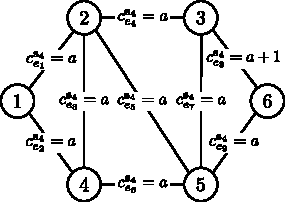
\includegraphics[width=\textwidth]{Chapter_II/MIN-MAX-DESC2-example/a}
		\caption{}
		\label{fig:minmaxexample:a}
	\end{subfigure}
	\hfill
	\begin{subfigure}[b]{0.3\textwidth}
		\includegraphics[width=\textwidth]{Chapter_II/MIN-MAX-DESC2-example/b}
		\caption{}
		\label{fig:minmaxexample:b}
	\end{subfigure}
	\hfill\null
	\caption{
		Dyskretne scenariusze $\textbf{s}_{4}$, $\textbf{s}_{5}$ dla grafu nieskierowanego $G = \left( V, E \right)$, $V = \left\{ 1, 2, \dots, 6 \right\}$, $E = \left\{ e_{i} : i \in \left\{ 1, \dots, 9 \right\} \right\}$.
		Dla tak określonych scenariuszy dłużej już nie zachodzi własność: $\forall e \in E : c^{\textbf{s}_{4}}_{e} \leqslant c^{\textbf{s}_{5}}_{e}$.
	}
	\label{fig:minmaxexample}
\end{figure}

Problem jest tym bardziej widoczny, im większe różnice będą zachodzić pomiędzy poszczególnymi scenariuszami.
Za przykład niech posłuży nam ilustracja \ref{fig:minmaxexample2}, gdzie pomimo występowania nadal jedynie dwóch scenariuszy, opieranie się na dotychczasowej intuicji policzenia optymalnych rozwiązań dla każdego z~nich i~wybraniu jednego, prowadzi do znacznie poważniejszych błędów, niż miało to miejsce w~poprzednim przykładzie, gdzie pomimo zastosowania błędnej logiki, otrzymaliśmy poprawny rezultat.
Wprowadźmy kolejne scenariusze: $\textbf{s}_{6} = \left[ 0, 0, 2^{n}, 2^{n}, 1, 1, 1, 1 \right]$ oraz $\textbf{s}_{7} = \left[ 2^{n}, 2^{n}, 0, 0, 1, 1, 1, 1 \right]$, gdzie $n$ jest dowolne\footnote{
	Chcemy aby funkcje zmiennej $n$ przyjmowały wartość większą od jedynki, co w~przypadku funkcji wykładniczej jest spełnione dla dowolnego $n \in \NN^{+}$.
}.

\begin{figure}[!htbp]
	\null\hfill
	\begin{subfigure}[b]{0.3\textwidth}
		\includegraphics[width=\textwidth]{Chapter_II/MIN-MAX-DESC3-example/a}
		\caption{}
		\label{fig:minmaxexample2:a}
	\end{subfigure}
	\hfill
	\begin{subfigure}[b]{0.3\textwidth}
		\includegraphics[width=\textwidth]{Chapter_II/MIN-MAX-DESC3-example/b}
		\caption{}
		\label{fig:minmaxexample2:b}
	\end{subfigure}
	\hfill\null
	\caption{
		Skrajny przykład problemu \textsc{Discrete Min-Max Spanning Tree}, gdzie optymalne rozwiązania dla poszczególnych scenariuszy okazują się być bardzo złe (dla dużych $n$) w~porównaniu z~rozwiązaniem głównego problemu.
		Podobny przykład~\cite[$429$--$430$]{minmaxSurvey} można skonstruować dla minimaksowego problemu najkrótszej ścieżki.
	}
	\label{fig:minmaxexample2}
\end{figure}

Optymalnymi rozwiązaniami dla poszczególnych scenariuszy są oczywiście: $T^{\ast}_{\textbf{s}_{6}} = \left\{ e_{1}, e_{2}, e_{6}, e_{7} \right\}$, o~całkowitym koszcie równym $2$, oraz $T^{\ast}_{\textbf{s}_{7}} = \left\{ e_{3}, e_{4}, e_{6}, e_{7} \right\}$, gdzie $v \left( \textbf{s}_{7}, x^{\ast}_{\textbf{s}_{7}} \right)$ ma tą samą wartość co poprzednie rozwiązanie\footnote{
	Z oznaczeniem $v \left( \textbf{s}, \textbf{x} \right)$ spotkaliśmy się już wcześniej, przy omawianiu tabeli \ref{tab:minmaxexample}, gdzie wyrażenie to oznaczało całkowity koszt dopuszczalnego rozwiązania problemu optymalizacyjnego dla zadanego scenariusza $\textbf{s}$ oraz wybranego zbioru krawędzi, reprezentowanego przez wektor $\textbf{x}$.
	Analogicznie poprzez $v \left( \textbf{s}, x^{\ast}_{\textbf{s}} \right)$ oznaczać będziemy koszt \textbf{optymalnego} rozwiązania dla scenariusza $\textbf{s}$, gdzie $x^{\ast}_{\textbf{s}}$ to binarny wektor reprezentujący optymalne rozwiązanie dla danego scenariusza ($T^{\ast} = \left\{ e : x_{e} = 1 \right\}$).
	Często będziemy skracać ten zapis do $v^{\ast}_{\textbf{s}}$.}.
Oczywiście po podstawieniu otrzymanych danych do wzoru: $\min_{\textbf{x} \in X^{\ast}} \max_{\textbf{s} \in \mathcal{S}} v \left( \textbf{x}, \textbf{s} \right)$, gdzie $X^{\ast} = \left\{ \textbf{x}^{\ast}_{\textbf{s}_{6}}, \textbf{x}^{\ast}_{\textbf{s}_{7}} \right\}$ otrzymamy:

\begin{equation*}
	\min \left\{ \max_{ \mathclap{\textbf{s} \in \mathcal{S}}} v \left( \textbf{x}^{\ast}_{\textbf{s}_{6}}, \textbf{s} \right), \max_{\mathclap{\textbf{s} \in \mathcal{S}}} v \left( \textbf{x}^{\ast}_{\textbf{s}_{7}}, \textbf{s} \right)  \right\} = \min \left\{ \max \left\{ v \left( \textbf{x}^{\ast}_{\textbf{s}_{6}}, \textbf{s}_{6} \right), v \left( \textbf{x}^{\ast}_{\textbf{s}_{6}}, \textbf{s}_{7} \right) \right\}, \max \left\{ v \left( \textbf{x}^{\ast}_{\textbf{s}_{7}}, \textbf{s}_{6} \right), v \left( \textbf{x}^{\ast}_{\textbf{s}_{7}}, \textbf{s}_{7} \right) \right\} \right\}\text{.}
\end{equation*}

Łatwo zauważyć, że $v \left( \textbf{x}^{\ast}_{\textbf{s}_{6}}, \textbf{s}_{6} \right) < v \left( \textbf{x}^{\ast}_{\textbf{s}_{6}}, \textbf{s}_{7} \right)$ oraz $v \left( \textbf{x}^{\ast}_{\textbf{s}_{7}}, \textbf{s}_{7} \right) < v \left( \textbf{x}^{\ast}_{\textbf{s}_{7}}, \textbf{s}_{6} \right)$. Stąd:

\begin{eqnarray}
	\max \left\{ v \left( \textbf{x}^{\ast}_{\textbf{s}_{6}}, \textbf{s}_{6} \right), v \left( \textbf{x}^{\ast}_{\textbf{s}_{6}}, \textbf{s}_{7} \right) \right\} = v \left( \textbf{x}^{\ast}_{\textbf{s}_{6}}, \textbf{s}_{7} \right) = 2 \cdot 2^{n} + 2 = 2^{n+1} + 2\text{,} \\
	\max \left\{ v \left( \textbf{x}^{\ast}_{\textbf{s}_{7}}, \textbf{s}_{6} \right), v \left( \textbf{x}^{\ast}_{\textbf{s}_{7}}, \textbf{s}_{7} \right) \right\} = v \left( \textbf{x}^{\ast}_{\textbf{s}_{7}}, \textbf{s}_{6} \right) = 2 \cdot 2^{n} + 2 = 2^{n+1} + 2\text{,}
\end{eqnarray}
a całe wyrażenie skraca się do $\min \left\{ 2^{n+1} + 2, 2^{n+1} + 2  \right\} = 2^{n+1} + 2$, podczas gdy optymalną wartością dla problemu \textsc{Min-Max Spanning Tree} dla tych scenariuszy wynosi $v \left( x^{\ast} \right) = v^{\ast} = 4$, gdzie $x^{\ast} = \left[ 0, 0, 0, 0, 1, 1, 1, 1 \right]$ (zbiór $T^{\ast} = \left\{ e_{5}, e_{6}, e_{7}, e_{8} \right\}$).
Uzyskaliśmy zatem błąd rzędu wykładniczego.



\subsection{Sposoby aproksymacji problemu}



Aby nie musieć uciekać się do rozwiązywania problemu \textsc{Min-Max} ze zbiorem scenariuszy $S$ prosto z~definicji tj.

\begin{itemize}
	\item dla każdego dopuszczalnego rozwiązania $\textbf{x} \in X$ wygenerować zbiór $V^{\textbf{x}}_{S} = \left\{ v \left( \textbf{x}, \textbf{s} \right) : \textbf{s} \in S \right\}$ (zawierający wartości rozwiązań dla ustalonego wektora $\textbf{x}$ dla wszystkich scenariuszy w~$S$),
	\item z~tak powstałego zbioru $\mathcal{V}^{X}_{S} = \left\{ \max_{y \in V^{\textbf{x}}_{S}} \left\{ y \right\} : \textbf{x} \in X  \right\}$ wybrać rozwiązanie $\textbf{x}^{\ast} \in X$, dla którego $v \left( \textbf{x}^{\ast}, S \right) = \min_{z \in \mathcal{V}^{X}_{S}} \left\{ z \right\}$,
\end{itemize}
możemy próbować aproksymować problem na podstawie jednego scenariusza, który jest składową wszystkich rozpatrywanych scenariuszy ~\cite{minmaxApprox}~\cite[$430$]{minmaxSurvey}.
Przyjrzyjmy się dwóm podejściom do rozpatrywanego przez nas problemu, w~obu przypadkach otrzymamy jego $k$-aproksymację, gdzie $k$ będzie liczbą scenariuszy, jakie bierzemy pod uwagę.
Choć będziemy skupiać się tylko na problemie \textsc{Min-Max Spanning Tree}, przedstawione dowody da się z~łatwością uogólnić na całą klasę problemów \textsc{Min-Max}.


\subsubsection{Uśrednianie scenariuszy}


Pierwszym, najprostszym do udowodnienia pomysłem jest potraktowanie problemu minimalizacyjnego $\mathcal{P}$ ze zbiorem scenariuszy $S$ ($\left| S \right| = k$) jako problemu z~pojedynczym scenariuszem, zdefiniowanym w~sposób podany w~poniższym twierdzeniu.

\begin{theorem}\label{th:minmaxavg}~\cite[$430$]{minmaxSurvey}
	Niech $\mathcal{I}$ będzie instancją problemu \textsc{Discrete Min-Max $\mathcal{P}$}.
	Niech problem zawiera $k$ scenariuszy w~zbiorze $S$ i~niech każdy $\textbf{s}_{j} \in S$ będzie zdefiniowany jako $\textbf{s}_{j} = \left[ c^{\textbf{s}_{j}}_{1}, \dots, c^{\textbf{s}_{j}}_{m} \right]$.
	Dodatkowo niech $\mathcal{I^{\prime}}$ będzie instancją problemu $\mathcal{P}$ z~jednym scenariuszem $\textbf{s}^{\prime}$, którego koszty są średnią kosztów scenariuszy $\textbf{s} \in S$.
	Wtedy, jeżeli istnieje optymalne rozwiązanie $\textbf{x}^{\prime}$ dla $\mathcal{I}^{\prime}$, to $\max_{\textbf{s} \in S} v \left( \textbf{x}^{\prime}, \textbf{s} \right) \leqslant k \cdot opt \left( \mathcal{I} \right)$, gdzie $opt \left( \mathcal{I} \right)$ oznacza optymalną wartość rozwiązania dla $\mathcal{I}$.
\end{theorem}

\begin{proof}~\cite[$430$]{minmaxSurvey}
	Koszty scenariusza $\textbf{s}^{\prime}$ dla $\mathcal{I}^{\prime}$ są zdefiniowane następująco:
	\begin{equation}
		c^{\textbf{s}^{\prime}}_{i} = \sum_{\mathclap{j = 1}}^{k} \frac{c_{i}^{\textbf{s}_{j}}}{k} \qquad \forall i \in \left\{ 1, \dots, m \right\}\text{.}
	\end{equation}
	
	Rozpisując wyrażenie $v \left( \textbf{x}, \textbf{s}^{\prime} \right) = \sum_{e \in E} x_{e} \cdot c^{\textbf{s}^{\prime}}_{e}$ otrzymujemy: $\sum_{e \in E} x_{e} \cdot \left( \sum_{j = 1}^{k} \frac{c_{e}^{\textbf{s}_{j}}}{k} \right) = \frac{1}{k} \cdot \sum_{j = 1}^{k} \sum_{e \in E} x_{e} \cdot c^{\textbf{s}_{j}}_{e} = \frac{1}{k} \cdot \sum_{\textbf{s} \in S} v \left( \textbf{x}, \textbf{s} \right)$.
	Pokażemy, że optymalne rozwiązanie $\textbf{x}^{\prime}$ dla scenariusza $\textbf{s}^{\prime}$ nie jest gorsze od optymalnego rozwiązania oryginalnego problemu (w przeciwnym wypadku rozważanie takiego scenariusza byłoby bezcelowe, gdyż nawet jego optymalne rozwiązanie było by gorsze od pożądanego).
	Mamy zatem:
	
	\begin{equation}
		L = v \left( \textbf{x}^{\prime}, \textbf{s}^{\prime} \right) = \min_{\mathclap{\textbf{x} \in X}} v \left( \textbf{x}, \textbf{s}^{\prime} \right) = \min_{ \mathclap{\textbf{x} \in X}} \frac{1}{k} \cdot \sum_{\textbf{s} \in S} v \left( \textbf{x}, \textbf{s} \right) \leqslant \min_{ \mathclap{\textbf{x} \in X}} \frac{1}{k} \cdot k \cdot \max_{\textbf{s} \in S} v \left( \textbf{x}, \textbf{s} \right) = \min_{ \mathclap{\textbf{x} \in X}} \max_{\textbf{s} \in S} v \left( \textbf{x}, \textbf{s} \right) = opt \left( \mathcal{I}\right)\text{.}
	\end{equation}
	
	W czasie obliczeń skorzystaliśmy z~własności $\sum_{\textbf{s} \in S} v \left( \textbf{x}, \textbf{s} \right) \leqslant k \cdot \max_{\textbf{s} \in S} v \left( \textbf{x}, \textbf{s} \right)$ (liczba scenariuszy $\left| S \right| = k$).
	Wartość $L$ nazywamy \textbf{dolnym ograniczeniem}.
	\textbf{Górnym ograniczeniem} na wartość rozwiązania jest oczywiście $\max_{\textbf{s} \in S} v \left( \textbf{x}^{\prime}, \textbf{s} \right) = U$.
	Próbując ograniczać otrzymaną wartość $U$ otrzymamy:
	
	\begin{eqnarray}
		opt \left( \mathcal{I} \right) = \min_{ \mathclap{\textbf{x} \in X}} \max_{\textbf{s} \in S} v \left( \textbf{x}, \textbf{s} \right) \leqslant \max_{\textbf{s} \in S} v \left( \textbf{x}^{\prime}, \textbf{s} \right) \leqslant \sum_{\textbf{s} \in S} v \left( \textbf{x}^{\prime}, \textbf{s} \right) = k \cdot \frac{1}{k} \cdot \sum_{\textbf{s} \in S} v \left( \textbf{x}^{\prime}, \textbf{s} \right) = k \cdot L \leqslant k \cdot opt \left( \mathcal{I} \right)\text{,}
	\end{eqnarray}
	gdzie w~dwóch ostatnich równościach skorzystaliśmy z~tego, że $L = \min_{ \textbf{x} \in X} \frac{1}{k} \cdot \sum_{\textbf{s} \in S} v \left( \textbf{x}, \textbf{s} \right) = \frac{1}{k} \cdot \sum_{\textbf{s} \in S} v \left( \textbf{x}^{\prime}, \textbf{s} \right)$ oraz, że wcześniej udowodniliśmy nierówność $L \leqslant opt \left( \mathcal{I} \right)$.
	Pokazaliśmy zatem, że $\max_{\textbf{s} \in S} v \left( \textbf{x}^{\prime}, \textbf{s} \right) \leqslant k \cdot opt \left( \mathcal{I} \right)$, co oznacza, że wybierając optymalne rozwiązanie $\textbf{x}^{\prime}$ dla scenariusza $\textbf{s}^{\prime}$, w~najgorszym możliwym przypadku (wystąpienia takiego scenariusza, że wartość rozwiązania dla wybranego $\textbf{x}^{\prime}$ będzie najbardziej oddalona od minimum) otrzymane rozwiązanie nie będzie gorsze niż $k$-krotność wartości optymalnej.
\end{proof}


\subsubsection{Scenariusz najgorszych wartości}


Scenariuszem najgorszych wartości będziemy nazywać taki scenariusz, którego każdy koszt, który definiuje, jest największym z~możliwych, odpowiadających mu, kosztów scenariuszy, z~których ten scenariusz powstaje.
Innymi słowy, powracając do rysunku \ref{fig:minmaxexample2}, jeżeli mamy dwa scenariusze: $\textbf{s}_{6} = \left[ 0, 0, 2^{n}, 2^{n}, 1, 1, 1, 1 \right]$ oraz $\textbf{s}_{7} = \left[ 2^{n}, 2^{n}, 0, 0, 1, 1, 1, 1 \right]$, to scenariuszem najgorszych wartości będzie scenariusz $s^{\prime} = \left[ 2^{n}, 2^{n}, 2^{n}, 2^{n}, 1, 1, 1, 1 \right]$ --- tak samo jak w~przypadku ciągłym, gdy najgorszy z~możliwych scenariuszy był definiowany za pomocą $\overline{s}$, tak wszystkie koszty scenariusza $s^{\prime}$ są nie mniejsze niż odpowiadające im wartości w~scenariuszach pozostałych.
Co więcej, jeżeli wykorzystalibyśmy tak stworzony scenariusz $s^{\prime}$ do rozwiązania problemu przedstawionego na ilustracji \ref{fig:minmaxexample2}, otrzymalibyśmy rozwiązanie optymalne, podobnie jak miałoby to miejsce w~przypadku ciągłym.
Pokażemy jednak, że --- pomimo obiecującego wyniku --- taka próba podejścia do problemów \textsc{Min-Max} nie zapewnia nam optymalnego rozwiązania, a~co najwyżej jego $k$-aproksymację, podobnie jak poprzednio zaprezentowana metoda.

\begin{theorem}\label{th:minmaxworst}~\cite[$430$]{minmaxSurvey}
	Niech $\mathcal{I}$ będzie instancją problemu \textsc{Discrete Min-Max $\mathcal{P}$}.
	Niech problem zawiera $k$ scenariuszy w~zbiorze $S$ i~niech każdy $\textbf{s} \in S$ będzie zdefiniowany jako $\textbf{s} = \left[ c^{\textbf{s}}_{1}, \dots, c^{\textbf{s}}_{m} \right]$.
	Dodatkowo niech $\mathcal{I^{\prime}}$ będzie instancją problemu $\mathcal{P}$ z~pojedynczym scenariuszem najgorszych wartości $\textbf{s}^{\prime}$.
	Wtedy, jeżeli istnieje optymalne rozwiązanie $\textbf{x}^{\prime}$ dla $\mathcal{I}^{\prime}$, to $\max_{\textbf{s} \in S} v \left( \textbf{x}^{\prime}, \textbf{s} \right) \leqslant k \cdot opt \left( \mathcal{I} \right)$, gdzie $opt \left( \mathcal{I} \right)$ oznacza optymalną wartość rozwiązania dla $\mathcal{I}$.
\end{theorem}

\begin{proof}~\cite[$430$]{minmaxSurvey}
	Koszty scenariusza $\textbf{s}^{\prime}$ dla $\mathcal{I}^{\prime}$ są zdefiniowane następująco:
	
	\begin{equation}
		c^{\textbf{s}^{\prime}}_{i} = \max_{\mathclap{\textbf{s} \in S}} c^{\textbf{s}}_{i} \qquad \forall i \in \left\{ 1, \dots, m \right\}\text{.}
	\end{equation}
	
	Pokażemy ciąg przekształceń, który da nam górne oszacowanie na wartość wyrażenia $ \max_{\textbf{s} \in S} v \left( \textbf{x}^{\prime}, \textbf{s} \right)$.
	Niech $\textbf{x}^{\ast}$ będzie optymalnym rozwiązaniem oryginalnego problemu $\mathcal{I}$:
	
	\begin{equation}
		\max_{\mathclap{\textbf{s} \in S}} v \left( \textbf{x}^{\prime}, \textbf{s} \right) \leqslant \sum_{\mathclap{i = 1}}^{m} c_{i}^{\textbf{s}^{\prime}} \cdot x_{i}^{\prime} \leqslant \sum_{\mathclap{i = 1}}^{m} c_{i}^{\textbf{s}^{\prime}} \cdot x_{i}^{\ast} \leqslant \sum_{\mathclap{i = 1}}^{m} \sum_{\mathclap{\textbf{s} \in S}} c_{i}^{\textbf{s}} \cdot x_{i}^{\ast} =  \sum_{\mathclap{\textbf{s} \in S}} \sum_{\mathclap{i = 1}}^{m} c_{i}^{\textbf{s}} \cdot x_{i}^{\ast} \leqslant k \cdot \max_{\mathclap{\textbf{s} \in S}} \sum_{\mathclap{i = 1}}^{m} c_{i}^{\textbf{s}} \cdot x_{i}^{\ast} = k \cdot opt \left( \mathcal{I} \right)\text{.}
	\end{equation}
	
	Chcąc dokładniej przyjrzeć się przeprowadzonemu przez nas rozumowaniu:
	
	\begin{itemize}
		\item $\max_{\textbf{s} \in S} v \left( \textbf{x}^{\prime}, \textbf{s} \right) = \sum_{i = 1}^{m} c_{i}^{\textbf{s}} \cdot x_{i}^{\prime} \leqslant \sum_{i = 1}^{m} c_{i}^{\textbf{s}^{\prime}} \cdot x_{i}^{\prime}$ otrzymujemy prosto z~definicji kosztów scenariusza $s^{\prime}$ --- dla każdego $i \in \left\{ 1, \dots, m \right\}$ zachodzi $c_{i}^{\textbf{s}} \leqslant \max_{\textbf{s} \in S} c^{\textbf{s}}_{i} = c_{i}^{\textbf{s}^{\prime}}$, zaś reszta wyrażenia nie ulega zmianie,
		\item $\sum_{i = 1}^{m} c_{i}^{\textbf{s}^{\prime}} \cdot x_{i}^{\prime} \leqslant \sum_{i = 1}^{m} c_{i}^{\textbf{s}^{\prime}} \cdot x_{i}^{\ast}$ --- rozwiązanie, opisywane przez wektor $\textbf{x}^{\prime}$, jest optymalne dla scenariusza z~kosztami $c_{i}^{\textbf{s}^{\prime}}$, zatem każde inne rozwiązanie jest nie lepsze od niego ($\textbf{x}^{\ast}$ jest optymalne dla kosztów oryginalnych, nie dla tych, które występują w~nierówności),
		\item $\sum_{i = 1}^{m} c_{i}^{\textbf{s}^{\prime}} \cdot x_{i}^{\ast} \leqslant \sum_{i = 1}^{m} \sum_{\textbf{s} \in S} c_{i}^{\textbf{s}} \cdot x_{i}^{\ast}$ w~oczywisty sposób wynika z~faktu, że dla każdego $i \in \left\{ 1, \dots, m \right\}$ zachodzi $c_{i}^{\textbf{s}^{\prime}} = \max_{\textbf{s} \in S} c^{\textbf{s}}_{i} \leqslant \sum_{\textbf{s} \in S} c^{\textbf{s}}_{i}$,
		\item $\max_{\textbf{s} \in S} \sum_{i = 1}^{m} c_{i}^{\textbf{s}} \cdot x_{i}^{\ast}$ jest równe wartości rozwiązania dla najgorszego możliwego przypadku, zakładając, że podstawiane do wzoru rozwiązanie $\textbf{x}^{\ast}$ jest optymalne --- $ opt \left( \mathcal{I} \right)$.
	\end{itemize}
	
	Pokazaliśmy zatem, tak samo jak w~przypadku poprzedniego twierdzenia, że takie podejście do problemu \textsc{Min-Max} zapewnia nam jedynie $k$-aproksymację rozwiązania.
\end{proof}




\section{Problemy minimaksowe ze względną funkcją optymalności}




W poprzednim dziale rozważaliśmy problem, który możemy najłatwiej określić pytaniem: ,,Jakie wybrać rozwiązanie, aby w~najgorszym przypadku było ono najlepsze z~możliwych?''.
Skupiało się zatem ono tylko na niwelowaniu strat, których można było się spodziewać, nie zaś na faktycznym szukaniu rozwiązania, które byłoby możliwie bliskie optymalnego.
W~tym podrozdziale zmienimy nieco nasze podejście do postawionego problemu i~zadamy sobie pytanie: ,,Jakie rozwiązanie wybrać, aby w~najgorszym przypadku było ono tak blisko rozwiązania optymalnego, jak to tylko możliwe?''.
Aby to osiągnąć, wprowadzimy pojęcie \textbf{żalu} (ang. \textit{regret}).
Niech $v_{\textbf{s}}^{\ast}$ oznacza wartość optymalnego rozwiązania dla scenariusza $\textbf{s}$.
Wektorem zapewniającym to rozwiązanie optymalne, jest wektor $x^{\ast}_{\textbf{s}}$.
Oznacza to, że dla każdego innego wektora $\textbf{x} \neq \textbf{x}^{\ast}_{\textbf{s}}$ zachodzi $v \left( \textbf{x}, \textbf{s} \right) \geqslant v \left( \textbf{x}^{\ast}_{\textbf{s}}, \textbf{s} \right)$.
Różnicę tych dwóch wartości nazywamy żalem i~reprezentuje on stratę, jaką ponieśliśmy w~konsekwencji wyboru innego rozwiązania niż optymalne dla danego scenariusza.
Istotą problemu \textsc{Min-Max Regret}~\cite[$595$]{Kasperski2012} jest wybranie takiego rozwiązania $\textbf{x}$, aby zminimalizować tę różnicę dla wszystkich scenariuszy, w~szczególności dla tego najgorszego, bo to od niego zależy wynik poniższego wyrażenia:

\begin{equation}
	\min_{\mathclap{\textbf{x} \in X}} \max_{\mathclap{\textbf{s} \in S}} \left( v \left( \textbf{x}, \textbf{s} \right) - v \left( \textbf{x}^{\ast}_{\textbf{s}}, \textbf{s} \right) \right)\text{.}
\end{equation}

Możemy także rozpatrywać przypadek \textsc{Max-Min Regret}, którego definicja nieco różni się od tej podanej wyżej i~nie jest analogiczna do problemu \textsc{Max-Min}: $\min_{\textbf{x} \in X} \max_{\textbf{s} \in S} \left( v \left( \textbf{x}^{\ast}_{\textbf{s}}, \textbf{s} \right) - v \left( \textbf{x}, \textbf{s} \right) \right)$.
Tak samo jak w~przypadku poprzednich problemów, tutaj też możemy wyróżnić podział na scenariusze ciągłe oraz dyskretne.



\subsection{Przypadek dyskretny}



Tym razem zaczniemy od omówienia przypadku dyskretnego, gdyż --- jak się będziemy mogli przekonać --- wiele z~tego, co do tej pory powiedzieliśmy o~problemach \textsc{Min-Max}, powtórzy się dla problemów \textsc{Min-Max Regret}.
Podobnie jak to miało miejsce w~przypadku poprzedniej klasy problemów, zaczniemy od omówienia prostego przykładu, który przedstawia rysunek \ref{fig:minmaxregexample}, a~na którym zaznaczono optymalne rozwiązania dla problemu \textsc{Min-Max Regret Minimum Spanning Tree} dla dwóch scenariuszy: $\textbf{s}_{1}$ oraz $\textbf{s}_{2}$, natomiast w~tabeli \ref{tab:minmaxregexample2} --- $7$ przykładowych wyników, jakie daje zastosowanie różnych drzew rozpinających.
Już dwa pierwsze rozwiązania: $\textbf{x}_{1}$ oraz $\textbf{x}_{2}$ wskazują na to, że kierowanie się przy wyborze rozwiązania dla tego problemu tylko kryterium optymalności dla pojedynczego scenariusza jest błędne i~nie należy go stosować; obydwa rozwiązania są optymalne odpowiednio dla scenariuszy $\textbf{s}_{1}$ oraz $\textbf{s}_{2}$, lecz nie dają tego samego rezultatu przy rozpatrywaniu właściwego problemu.

\begin{figure}[!htbp]
	\null\hfill
	\begin{subfigure}[b]{0.35\textwidth}
		\includegraphics[width=\textwidth]{Chapter_II/MIN-MAX-REG-example/a}
		\caption{}
		\label{fig:minmaxregexample:a}
	\end{subfigure}
	\hfill
	\begin{subfigure}[b]{0.35\textwidth}
		\includegraphics[width=\textwidth]{Chapter_II/MIN-MAX-REG-example/b}
		\caption{}
		\label{fig:minmaxregexample:b}
	\end{subfigure}
	\hfill\null
	\caption{
		Dyskretne scenariusze $\textbf{s}_{1}$, $\textbf{s}_{2}$ dla grafu nieskierowanego $G = \left( V, E \right)$, $V = \left\{ 1, 2, \dots, 6 \right\}$, $E = \left\{ e_{i} : i \in \left\{ 1, \dots, 9 \right\} \right\}$.
		\textbf{(a)}~Optymalnym rozwiązaniem dla scenariusza $\textbf{s}_{1}$ jest zbiór wierzchołków $T^{\ast}_{\textbf{s}_{1}} = \left\{ e_{1}, e_{3}, e_{4}, e_{6}, e_{9} \right\}$, któremu odpowiada wektor $\textbf{x}^{\ast}_{\textbf{s}_{1}} = \left[ 1, 0, 1, 1, 0, 1, 0, 0, 1 \right]$.
		Wartość tego rozwiązania wynosi $v^{\ast}_{\textbf{s}_{1}} = 11$.
		\textbf{(b)}~Optymalnym rozwiązaniem dla scenariusza $\textbf{s}_{2}$ jest zbiór wierzchołków $T^{\ast}_{\textbf{s}_{2}} = \left\{ e_{1}, e_{3}, e_{4}, e_{6}, e_{8} \right\}$, któremu odpowiada wektor $\textbf{x}^{\ast}_{\textbf{s}_{2}} = \left[ 1, 0, 1, 1, 0, 1, 0, 1, 0 \right]$.
		Wartość tego rozwiązania wynosi $v^{\ast}_{\textbf{s}_{2}} = 25$.
	}
	\label{fig:minmaxregexample}
\end{figure}

\begin{table}[!htbp]
	\caption{
		Tabela przedstawiająca część z~osiągalnych rozwiązań dla problemu minimalnego drzewa rozpinającego dla scenariuszy $\textbf{s}_{1}$ oraz $\textbf{s}_{2}$ (\ref{fig:minmaxregexample:a} i~\ref{fig:minmaxregexample:b}), koszty dla każdego z~proponowanych rozwiązań dla podanych scenariuszy, poniesione straty względem optymalnych rozwiązań oraz wartość rozwiązania dla problemu \textsc{Min-Max Regret}.
		Wiersze w~tabeli zostały posortowane w~kolejności rosnących wartości rozwiązań.
	}
	\label{tab:minmaxregexample2}
	\centering
	\begin{tabular}{ccccccccccccccc}
		\cline{11-15}
		\multicolumn{2}{c}{}       &         &         &         &         &         &         &         &         & \multicolumn{5}{c}{Scenariusze}                                                                                                                                                                                             \\ \hline
		$X$              & $e_{1}$ & $e_{2}$ & $e_{3}$ & $e_{4}$ & $e_{5}$ & $e_{6}$ & $e_{7}$ & $e_{8}$ & $e_{9}$ & $v \left( \textbf{x}, \textbf{s}_{1} \right) $ & $r_{\textbf{s}_{1}}$  & $v \left( \textbf{x}, \textbf{s}_{2} \right) $ &  $r_{\textbf{s}_{2}}$ & $\max \left\{ r_{\textbf{s}_{1}}, r_{\textbf{s}_{2}} \right\} $ \\ \hline
		$\textbf{x}_{1}$ & $1$     & $0$     & $1$     & $1$     & $0$     & $1$     & $0$     & $0$	&	$1$	&	$11$	&	$0$	&	$26$	&	$1$	&	$1$	\\
		$\textbf{x}_{2}$ & $1$     & $0$     & $1$     & $1$     & $0$     & $1$     & $0$     & $1$	&	$0$	&	$13$	&	$2$	&	$25$	&	$0$	&	$2$	\\
		$\textbf{x}_{3}$ & $1$     & $0$     & $1$     & $0$     & $0$     & $1$     & $0$     & $1$	&	$1$	&	$13$	&	$2$	&	$26$	&	$1$	&	$2$	\\
		$\textbf{x}_{4}$ & $1$     & $0$     & $1$     & $0$     & $0$     & $1$     & $1$     & $0$	&	$1$	&	$12$	&	$1$	&	$28$	&	$3$	&	$3$	\\
		$\dots$ & $\dots$     & $\dots$     & $\dots$     & $\dots$     & $\dots$     & $\dots$     & $\dots$     & $\dots$	&	$\dots$	&	$\dots$	&	$\dots$	&	$\dots$	&	$\dots$	&	$\dots$	\\
		$\textbf{x}_{53}$ & $0$     & $1$     & $1$     & $0$     & $1$     & $0$     & $1$     & $1$	&	$0$	&	$25$	&	$14$	&	$35$	&	$10$	&	$14$	\\
		$\textbf{x}_{54}$ & $0$     & $1$     & $0$     & $0$     & $1$     & $1$     & $1$     & $1$	&	$0$	&	$26$	&	$15$	&	$38$	&	$13$	&	$15$	\\
		$\textbf{x}_{55}$ & $1$     & $1$     & $0$     & $0$     & $1$     & $0$     & $1$     & $1$	&	$0$	&	$26$	&	$15$	&	$37$	&	$12$	&	$15$	\\
		\hline
	\end{tabular}
\end{table}

\begin{figure}[!htbp]
	\null\hfill
	\begin{subfigure}[b]{0.3\textwidth}
		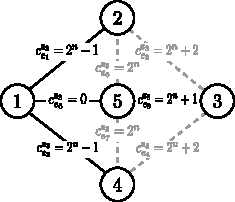
\includegraphics[width=\textwidth]{Chapter_II/MIN-MAX-REG2-example/a}
		\caption{}
		\label{fig:minmaxregexample2:a}
	\end{subfigure}
	\hfill
	\begin{subfigure}[b]{0.3\textwidth}
		\includegraphics[width=\textwidth]{Chapter_II/MIN-MAX-REG2-example/b}
		\caption{}
		\label{fig:minmaxregexample2:b}
	\end{subfigure}
	\hfill
	\begin{subfigure}[b]{0.3\textwidth}
		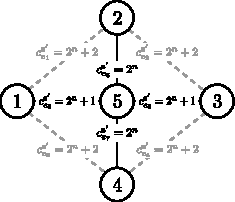
\includegraphics[width=\textwidth]{Chapter_II/MIN-MAX-REG2-example/c}
		\caption{}
		\label{fig:minmaxregexample2:c}
	\end{subfigure}
	\hfill\null
	\caption{
		Dyskretne scenariusze $\textbf{s}_{3}$, $\textbf{s}_{4}$ i~$\textbf{s}^{\prime}$ dla grafu nieskierowanego $G = \left( V, E \right)$, $V = \left\{ 1, 2, \dots, 5 \right\}$, $E = \left\{ e_{i} : i \in \left\{ 1, \dots, 8 \right\} \right\}$, gdzie $\textbf{s}^{\prime}$ jest sztucznie wygenerowanym scenariuszem najgorszych kosztów.
		\textbf{(a)}~Optymalne rozwiązanie $T^{\ast}_{\textbf{s}_{3}} = \left\{ e_{1}, e_{3}, e_{5}, e_{8} \right\}$ o~całkowitym koszcie $3 \cdot 2^{n} - 1$.
		\textbf{(b)}~Optymalne rozwiązanie $T^{\ast}_{\textbf{s}_{4}} = \left\{ e_{2}, e_{4}, e_{5}, e_{8} \right\}$ o~identycznym koszcie, co $v^{\ast}_{\textbf{s}_{3}}$.
		\textbf{(c)}~Optymalne rozwiązanie dla scenariusza $\textbf{s}^{\prime}$ o~kosztach $c_{i}^{\textbf{s}^{\prime}} = \max_{\textbf{s} \in S} c_{i}^{\textbf{s}}$.
		Koszt całkowity rozwiązania optymalnego wynosi $v \left( \textbf{x}^{\ast}_{\textbf{s}^{\prime}}, \textbf{s}^{\prime} \right) = 4 \cdot 2^{n} + 2$.
	}
	\label{fig:minmaxregexample2}
\end{figure}


\subsubsection{Aproksymacja rozwiązania}


Chcąc otrzymać aproksymację dla problemu \textsc{Min-Max Regret}, możemy odwołać się do udowodnionego twierdzenia \ref{th:minmaxavg} --- jego dowód przebiega analogicznie dla tej klasy problemów~\cite[propozycja $1$]{minmaxSurvey} i~zostanie tu pominięty.
Dużo ciekawszy okazuje się natomiast przypadek, w~którym tworzyliśmy dodatkowy scenariusz $s^{\prime}$, którego koszty definiowaliśmy jako $c^{\prime}_{i} = \max_{\textbf{s} \in S} c^{\textbf{s}}_{i} \; \forall i \in \left\{ 1, \dots, m \right\}$.
Pokażemy, że nawet dla dwóch scenariuszy (gdzie spodziewalibyśmy się wyniku co najwyżej $2$ razy gorszego niż optymalny) otrzymany rezultat jest dalece gorszy od spodziewanego.
Stwórzmy dwa scenariusze: $\textbf{s}_{3} = \left[ 2^{n} - 1, 2^{n} + 2, 2^{n} - 1, 2^{n} + 2, 0, 2^{n}, 2^{n}, 2^{n} + 1 \right]$ oraz $\textbf{s}_{4} = \left[ 2^{n} + 2, 2^{n} - 1, 2^{n} + 2, 2^{n} - 1, 2^{n} + 1, 2^{n}, 2^{n}, 0 \right]$, tak jak na rysunku \ref{fig:minmaxregexample2}.
Będziemy chcieli pokazać, że optymalna wartość rozwiązania problemu \textsc{Min-Max Regret Minimum Spanning Tree} dla takiej konfiguracji scenariuszy wynosi $0$, toteż każda inna wartość (różna od zera), jaką otrzymamy przy rozwiązywaniu problemu z~wykorzystaniem scenariusza $\textbf{s}^{\prime}$, będzie błędna (zgodnie z~twierdzeniem \ref{th:minmaxworst}: $\max_{\textbf{s} \in S} v \left( \textbf{x}^{\prime}, \textbf{s} \right) \leqslant k \cdot opt \left( \mathcal{I} \right)$, zatem w~przypadku, gdy $opt \left( \mathcal{I} \right) = 0$, gdzie $\mathcal{I}$ to instancja oryginalnego problemu, jedyne rozwiązanie $\textbf{x}^{\prime}$ dla scenariusza $\textbf{s}^{\prime}$, które spełnia tą nierówność, także musi mieć wartość równą $0$)\footnote{
	Rozpatrywane przez nas grafy nie posiadają ujemnych wag krawędzi.
}. 

Jak łatwo zauważyć, koszty obydwu scenariuszy dla problemu zostały tak dobrane, aby oba optymalne rozwiązania dla każdego scenariusza nie różniły się pod względem wartości, która wynosi $v^{\ast}_{\textbf{s}_{3}} = v^{\ast}_{\textbf{s}_{4}} = 3 \cdot 2^{n} - 1$.
Jest to o~tyle istotne, że podstawiając te dane do ogólnego wzoru, otrzymujemy:

\begin{equation}\label{eq:minmaxreg}
	\min_{\textbf{x} \in X} \max_{\textbf{s} \in \left\{ \textbf{s}_{3}, \textbf{s}_{4} \right\}} v \left( \textbf{x}, \textbf{s} \right) - v \left( \textbf{x}^{\ast}_{\textbf{s}}, \textbf{s} \right) = \min \left\{   \max_{\textbf{s} \in \left\{ \textbf{s}_{3}, \textbf{s}_{4} \right\}} v \left( \textbf{x}^{\ast}_{\textbf{s}_{3}}, \textbf{s} \right) - v \left( \textbf{x}^{\ast}_{\textbf{s}}, \textbf{s} \right), \max_{\textbf{s} \in \left\{ \textbf{s}_{3}, \textbf{s}_{4} \right\}} v \left( \textbf{x}^{\ast}_{\textbf{s}_{4}}, \textbf{s} \right) - v \left( \textbf{x}^{\ast}_{\textbf{s}}, \textbf{s} \right) \right\}\text{.}
\end{equation}

Na tym etapie możemy zauważyć, że bez względu na to, które rozwiązanie wybierzemy (czy $\textbf{x}^{\ast}_{\textbf{s}_{3}}$ czy $\textbf{x}^{\ast}_{\textbf{s}_{4}}$), dla obu rozpatrywanych scenariuszy otrzymamy identyczną wartość żalu (równą zeru).
Podstawiając dane do wzoru \ref{eq:minmaxreg}, otrzymamy zatem: $\min \left\{ \max \left\{ 0, 0 \right\} , \max \left\{ 0, 0 \right\} \right\} = 0$.
Innych rozwiązań nie rozpatrywaliśmy, gdyż z~samej definicji problemu \textsc{Min-Max Regret} wynika, że $\forall x \in X \; v \left( \textbf{x}, \textbf{s} \right) - v \left( \textbf{x}^{\ast}_{\textbf{s}}, \textbf{s} \right) \geqslant 0$, toteż wartości otrzymane dla pozostałych rozwiązań z~pewnością nie mogą być lepsze.

Zakładając, że analogiczne do \ref{th:minmaxworst} twierdzenie dla \textsc{Min-Max Regret} jest prawdziwe, spodziewamy się, że wartość optymalnego rozwiązania dla dodatkowego scenariusza $\textbf{s}^{\prime}$ będzie nie gorsza niż $k$-krotność powyżej otrzymanego rozwiązania (będzie równa $0$).
Z~rysunku \ref{fig:minmaxregexample2:c} natomiast jednoznacznie wynika, że rozwiązaniem dla tego scenariusza jest zbiór krawędzi $T^{\ast}_{\textbf{s}^{\prime}} = \left\{ e_{5}, e_{6}, e_{7}, e_{8} \right\}$ o~całkowitym koszcie równym $2^{n+2} + 2$, gdzie $\textbf{x}^{\ast}_{\textbf{s}^{\prime}} = \left[ 0, 0, 0, 0, 1, 1, 1, 1 \right]$, zaś po podstawieniu danych do wzoru otrzymamy:

\begin{gather*}
	\min_{\textbf{x} \in \left\{ x^{\ast}_{\textbf{s}^{\prime}} \right\}} \max_{\textbf{s} \in \left\{ \textbf{s}_{3}, \textbf{s}_{4} \right\}} v \left( \textbf{x}, \textbf{s} \right) - v \left( \textbf{x}^{\ast}_{\textbf{s}}, \textbf{s} \right) = \max_{\textbf{s} \in \left\{ \textbf{s}_{3}, \textbf{s}_{4} \right\}} v \left( x^{\ast}_{\textbf{s}^{\prime}}, \textbf{s} \right) - v \left( \textbf{x}^{\ast}_{\textbf{s}}, \textbf{s} \right) = \\ 
	= \max \left\{ v \left( x^{\ast}_{\textbf{s}^{\prime}}, \textbf{s}_{3} \right), v \left( x^{\ast}_{\textbf{s}^{\prime}}, \textbf{s}_{4} \right) \right\} - \left( 3 \cdot 2^{n} - 1 \right) = \max \left\{ 3 \cdot 2^{n} + 1, 3 \cdot 2^{n} + 1 \right\} - 3 \cdot 2^{n} + 1 = 2\text{.}
\end{gather*}

Wynikiem możemy dowolnie manipulować --- przykładem takiej manipulacji są scenariusze $\textbf{s}^{\prime}_{3}$, $\textbf{s}^{\prime}_{4}$ oraz $\textbf{s}^{\prime\prime}$, przedstawione (wraz z~optymalnymi rozwiązaniami dla każdego z~nich) na rysunkach \ref{fig:minmaxregexample3:a}, \ref{fig:minmaxregexample3:b} i~\ref{fig:minmaxregexample3:c}, gdzie optymalną wartością rozwiązania problemu \textsc{Min-Max Regret} dla tych pierwszych jest ponownie wartość $0$, zaś dla trzeciego z~nich: $2^{n+1} \cdot \left( 2^{n} - 1\right)$.

\begin{figure}[!htbp]
	\null\hfill
	\begin{subfigure}[b]{0.3\textwidth}
		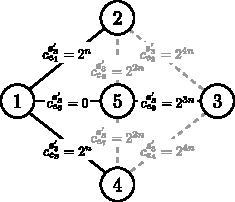
\includegraphics[width=\textwidth]{Chapter_II/MIN-MAX-REG3-example/a}
		\caption{}
		\label{fig:minmaxregexample3:a}
	\end{subfigure}
	\hfill
	\begin{subfigure}[b]{0.3\textwidth}
		\includegraphics[width=\textwidth]{Chapter_II/MIN-MAX-REG3-example/b}
		\caption{}
		\label{fig:minmaxregexample3:b}
	\end{subfigure}
	\hfill
	\begin{subfigure}[b]{0.3\textwidth}
		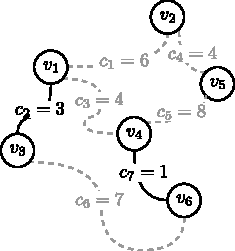
\includegraphics[width=\textwidth]{Chapter_II/MIN-MAX-REG3-example/c}
		\caption{}
		\label{fig:minmaxregexample3:c}
	\end{subfigure}
	\hfill\null
	\caption{
		Scenariusze $\textbf{s}_{3}^{\prime}$ i~$\textbf{s}_{4}^{\prime}$, dla których scenariusz najgorszych kosztów $\textbf{s}^{\prime\prime}$ daje bardzo złe rozwiązanie.
		\textbf{(a)}~Minimalne drzewo rozpinające dla scenariusza $\textbf{s}_{3}^{\prime}$ o~całkowitym koszcie $v^{\ast}_{\textbf{s}_{3}^{\prime}} = 2^{3n} + 2 \cdot 2^{n}$.
		\textbf{(b)}~Minimalne drzewo rozpinające dla scenariusza $\textbf{s}_{4}^{\prime}$ o~takim samym koszcie.
		\textbf{(c)}~Optymalne drzewo rozpinające dla scenariusza $\textbf{s}^{\prime\prime}$.
	}
	\label{fig:minmaxregexample3}
\end{figure}

Pokazaliśmy zatem, że w~tym przypadku nie możemy zastosować analogicznego twierdzenia.



\subsection{Przypadek ciągły}



Zacznijmy od następującego twierdzenia:

\begin{theorem}\label{th:intminmaxreg}~\cite[$431$]{minmaxSurvey}
	Niech dany będzie problem minimalizacyjny $\mathcal{P}$.
	Niech $\underline{\textbf{s}}$ i~$\overline{\textbf{s}}$ będą krytycznymi scenariuszami (odpowiednio najgorszym i~najlepszym), definiującymi przestrzeń scenariuszy $S$.
	Wartość żalu dla dowolnego rozwiązania $\textbf{x} \in X$ jest największa dla, zależnego od $\textbf{x}$, scenariusza $\textbf{s}^{-} \left( \textbf{x} \right)$, którego koszty są zdefiniowane następująco:
	
	\begin{equation}
		c^{\textbf{s}^{-} \left( \textbf{x} \right)}_{i} = \left\{\begin{matrix}
			c^{\overline{\textbf{s}}}_{i} & \text{gdy $e_{i}$ należy do rozwiązania ($x_{i} = 1$),}\\ 
			c^{\underline{\textbf{s}}}_{i} &  \text{w przeciwnym przypadku ($x_{i} = 0$),}
		\end{matrix}\right. \qquad \forall i \in \left\{ 1, 2, \dots, m \right\}\text{.}
	\end{equation}
\end{theorem}

\begin{proof}~\cite[$431$]{minmaxSurvey}
	Dla danego rozwiązania $\textbf{x} \in X$ niech będzie dany zbiór $\mathbb{1} \left( \textbf{x} \right) = \left\{ i : i \in \left\{ 1, \dots, m \right\} \; \wedge \; x_{i} = 1 \right\}$.
	Wartość żalu dla scenariusza $\textbf{s} \in S$ i~dowolnego rozwiązania $\textbf{x}$ wynosi:
	
	\begin{gather*}
		R \left( \textbf{x}, \textbf{s} \right) = v \left( \textbf{x}, \textbf{s} \right) - v^{\ast}_{\textbf{s}} \overset{\left( 1 \right)}{=} \sum_{\mathclap{i \in \mathbb{1} \left( \textbf{x} \right) \setminus \mathbb{1} \left( \textbf{x}^{\ast}_{\textbf{s}} \right)}} c_{i}^{\textbf{s}} \quad - \quad \sum_{\mathclap{i \in \mathbb{1} \left( \textbf{x}^{\ast}_{\textbf{s}} \right) \setminus \mathbb{1} \left( \textbf{x} \right)}} c_{i}^{\textbf{s}} \quad \overset{\left( 2 \right)}{\leqslant} \quad \sum_{\mathclap{i \in \mathbb{1} \left( \textbf{x} \right) \setminus \mathbb{1} \left( \textbf{x}^{\ast}_{\textbf{s}} \right)}} c^{\overline{\textbf{s}}}_{i} \quad - \quad \sum_{\mathclap{i \in \mathbb{1} \left( \textbf{x}^{\ast}_{\textbf{s}} \right) \setminus \mathbb{1} \left( \textbf{x} \right)}} c^{\underline{\textbf{s}}}_{i} \overset{\left( 3 \right)}{=} \\ 
		\overset{\left( 3 \right)}{=} v \left( \textbf{x}, \textbf{s}^{-} \left( \textbf{x} \right) \right) - v \left( \textbf{x}^{\ast}_{\textbf{s}}, \textbf{s}^{-} \left( \textbf{x} \right) \right) \overset{\left( 4 \right)}{\leqslant} v \left( \textbf{x}, \textbf{s}^{-} \left( \textbf{x} \right) \right) - v \left( \textbf{x}^{\ast}_{\textbf{s}^{-} \left( \textbf{x} \right)}, \textbf{s}^{-} \left( \textbf{x} \right) \right) = \\ 
		= v \left( \textbf{x}, \textbf{s}^{-} \left( \textbf{x} \right) \right) - v^{\ast}_{\textbf{s}^{-} \left( \textbf{x} \right)} = R \left( \textbf{x}, \textbf{s}^{-} \left( \textbf{x} \right) \right)\text{,}
	\end{gather*}
	co dowodzi poprawności twierdzenia.
	Aby lepiej zrozumieć ciąg logicznego rozumowania jaki został podjęty, skupimy się teraz na kilku, kluczowych dla dowodu, przekształceniach.
	
	\begin{itemize}
		\item[$\left( 1 \right)$] Niech $\mathbb{0} \left( \textbf{x} \right) = \left\{ i : i \in \left\{ 1, \dots, m \right\} \; \wedge \; x_{i} = 0 \right\}$.
		Łatwo zauważyć, że $\mathbb{0} \left( \textbf{x} \right)$ i~$\mathbb{1} \left( \textbf{x} \right)$ są rozłączne, zaś ich suma $\mathbb{0} \left( \textbf{x} \right) \cup \mathbb{1} \left( \textbf{x} \right)$ generuje cały zbiór $\left\{ i : i \in \left\{ 1, \dots, m \right\} \right\}$.
		Rozpisując wzór na wartość rozwiązania $\textbf{x}$ dla danego scenariusza $\textbf{s}$ mamy: $v \left( \textbf{x}, \textbf{s} \right) = \sum_{e_{i} \in E} x_{i} \cdot c^{\textbf{s}}_{i} = \sum_{i \in \left( \mathbb{0} \cup \mathbb{1} \right) \left( \textbf{x} \right)} x_{i} \cdot c^{\textbf{s}}_{i} = \sum_{i \in \mathbb{0} \left( \textbf{x} \right)} 0 \cdot c^{\textbf{s}}_{i} + \sum_{i \in \mathbb{1} \left( \textbf{x} \right)} 1 \cdot c^{\textbf{s}}_{i} = \sum_{i \in \mathbb{1} \left( \textbf{x} \right)} c^{\textbf{s}}_{i}$.
		Analogicznie możemy postąpić dla $v^{\ast}_{\textbf{s}} = v \left( \textbf{x}^{\ast}_{\textbf{s}}, \textbf{s} \right) = \sum_{i \in \mathbb{1} \left( \textbf{x}^{\ast}_{\textbf{s}} \right)} c^{\textbf{s}}_{i}$.
		Zauważmy, że w~wyrażeniu $v \left( \textbf{x}, \textbf{s} \right) - v^{\ast}_{\textbf{s}}$ wszystkie elementy sumy, które należą do obu zbiorów, zredukują się:
		
		\begin{gather*}
			v \left( \textbf{x}, \textbf{s} \right) - v^{\ast}_{\textbf{s}} = \sum_{\mathclap{i \in \mathbb{1} \left( \textbf{x} \right)}} c^{\textbf{s}}_{i} - \sum_{\mathclap{i \in \mathbb{1} \left( \textbf{x}^{\ast}_{\textbf{s}} \right)}} c^{\textbf{s}}_{i} = \left( \quad \; \; \sum_{\mathclap{i \in \mathbb{1} \left( \textbf{x} \right) \setminus \mathbb{1} \left( \textbf{x}^{\ast}_{\textbf{s}} \right) }} c^{\textbf{s}}_{i} \; + \; \sum_{\mathclap{i \in \mathbb{1} \left( \textbf{x}^{\ast}_{\textbf{s}} \right) }} c^{\textbf{s}}_{i} \; - \; \sum_{\mathclap{i \in \mathbb{1} \left( \textbf{x}^{\ast}_{\textbf{s}} \right) \setminus \mathbb{1} \left( \textbf{x} \right) }} c^{\textbf{s}}_{i} \quad \; \; \right) - \sum_{\mathclap{i \in \mathbb{1} \left( \textbf{x}^{\ast}_{\textbf{s}} \right) }} c^{\textbf{s}}_{i} = \\ 
			= \quad \sum_{\mathclap{i \in \mathbb{1} \left( \textbf{x} \right) \setminus \mathbb{1} \left( \textbf{x}^{\ast}_{\textbf{s}} \right) }} c^{\textbf{s}}_{i} \quad - \quad \sum_{\mathclap{i \in \mathbb{1} \left( \textbf{x}^{\ast}_{\textbf{s}} \right) \setminus \mathbb{1} \left( \textbf{x} \right) }} c^{\textbf{s}}_{i}\text{.}
		\end{gather*}
		
		\item[$\left( 2 \right)$] Łatwo zauważyć, że suma po prawej stronie nierówności jest większa ze względu na definicje kosztów scenariuszy $\overline{\textbf{s}}$ oraz $\underline{\textbf{s}}$ ($\sum_{i \in \mathbb{1} \left( \textbf{x} \right) \setminus \mathbb{1} \left( \textbf{x}^{\ast}_{\textbf{s}} \right)} c_{i}^{\textbf{s}} \leqslant \sum_{i \in \mathbb{1} \left( \textbf{x} \right) \setminus \mathbb{1} \left( \textbf{x}^{\ast}_{\textbf{s}} \right)} c_{i}^{\overline{\textbf{s}}}$ oraz $\sum_{i \in \mathbb{1} \left( \textbf{x}^{\ast}_{\textbf{s}} \right) \setminus \mathbb{1} \left( \textbf{x} \right)} c_{i}^{\textbf{s}} \geqslant \sum_{i \in \mathbb{1} \left( \textbf{x}^{\ast}_{\textbf{s}} \right) \setminus \mathbb{1} \left( \textbf{x} \right)} c_{i}^{\underline{\textbf{s}}}$). 
		\item[$\left( 3 \right)$] Przeprowadzone rozumowanie jest analogiczne do tego z~punktu $\left( 2 \right)$ --- na uwagę zasługuje fakt, iż:
		
		\begin{equation*}
			\sum_{\mathclap{i \in \mathbb{1} \left( \textbf{x} \right) \setminus \mathbb{1} \left( \textbf{x}^{\ast}_{\textbf{s}} \right)}} c^{\overline{\textbf{s}}}_{i} \quad - \quad \sum_{\mathclap{i \in \mathbb{1} \left( \textbf{x}^{\ast}_{\textbf{s}} \right) \setminus \mathbb{1} \left( \textbf{x} \right)}} c^{\underline{\textbf{s}}}_{i} \quad = \quad \sum_{\mathclap{i \in \mathbb{1} \left( \textbf{x} \right) \setminus \mathbb{1} \left( \textbf{x}^{\ast}_{\textbf{s}} \right)}} c^{\textbf{s}^{-}}_{i} \quad - \quad \sum_{\mathclap{i \in \mathbb{1} \left( \textbf{x}^{\ast}_{\textbf{s}} \right) \setminus \mathbb{1} \left( \textbf{x} \right)}} c^{\textbf{s}^{-}}_{i}\text{,}
		\end{equation*}
		co bezpośrednio wynika z~definicji scenariusza $\textbf{s}^{-} \left( \textbf{x} \right)$ --- dla wszystkich elementów pierwszej sumy (indeksowanej po $i \in \mathbb{1} \left( \textbf{x} \right) \setminus \mathbb{1} \left( \textbf{x}^{\ast}_{\textbf{s}} \right)$) koszty dla tych elementów $x_{i}$ przyjmują wartość $c^{\overline{\textbf{s}}}_{i}$ ($x_{i} = 1$).
		Analogicznie druga suma jest indeksowana po $i$, które w~szczególności nie należą do zbioru $\mathbb{1} \left( \textbf{x} \right)$, tak więc dla każdego elementu tej sumy spełniony jest warunek $x_{i} = 0$.
		Poczyniwszy tę obserwację, dalsze przekształcanie formuły odbywa się identycznie, jak przedstawiono w~kroku $\left( 2 \right)$.
		\item[$\left( 4 \right)$] Wynika bezpośrednio z~właściwości optymalnego rozwiązania $\textbf{x}^{\ast}_{\textbf{s}^{-} \left( \textbf{x} \right)}$ dla scenariusza $\textbf{s}^{-} \left( \textbf{x} \right)$:
		
		\begin{equation*}
			v \left( \textbf{x}^{\ast}_{\textbf{s}}, \textbf{s}^{-} \left( \textbf{x} \right) \right) \geqslant v \left( \textbf{x}^{\ast}_{\textbf{s}^{-} \left( \textbf{x} \right)}, \textbf{s}^{-} \left( \textbf{x} \right) \right) = v^{\ast}_{\textbf{s}^{-} \left( \textbf{x} \right)}\text{.}
		\end{equation*}
	\end{itemize}
\end{proof}

Udowodniliśmy zatem, że dla dowolnego rozwiązania $\textbf{x} \in X$ wartość $R \left( \textbf{x}, \textbf{s} \right) = v \left( \textbf{x}, \textbf{s} \right) - v^{\ast}_{\textbf{s}}$ osiąga swoje maksimum dla $\textbf{s} = \textbf{s}^{-} \left( \textbf{x} \right)$.
W~oparciu o~twierdzenie \ref{th:intminmaxreg} możemy wyciągnąć następujący wniosek, od którego tylko krok dzieli nas od podania metody na rozwiązywanie zagadnienia \textsc{Interval Min-Max Regret}.

\begin{corollary}
	Dla problemu \textsc{Interval Min-Max Regret $\mathcal{P}$}, gdzie $\mathcal{P}$ jest problemem minimalizacyjnym, optymalnym rozwiązaniem $\textbf{x}^{\ast}$ jest jedno z~rozwiązań $\textbf{x} \in X$ dla scenariusza $\textbf{s}^{-} \left( \textbf{x} \right)$.
\end{corollary}

Znaczy to dla nas tyle, że zamiast rozwiązywać problem z~definicji: $\min_{\textbf{x} \in X} \max_{\textbf{s} \in S} R \left( \textbf{x}, \textbf{s} \right)$, możemy równoważnie rozważać problem $\min_{\textbf{x} \in X} R \left( \textbf{x}, \textbf{s}^{-} \left( \textbf{x} \right) \right)$.
Tak więc, jeśli istnieje optymalne rozwiązanie problemu $\min_{\textbf{x} \in X} R \left( \textbf{x}, \textbf{s}^{-} \left( \textbf{x} \right) \right)$, jest ono także optymalnym rozwiązaniem dla $\min_{\textbf{x} \in X} \max_{\textbf{s} \in S} R \left( \textbf{x}, \textbf{s} \right)$.

Choć powyższe twierdzenie da się łatwo uogólnić na klasę problemów \textsc{Min-Max Regret} (co też uczyniliśmy), pierwotny pomysł wywodzi się z~rozważań nad problemem \textsc{Min-Max Regret Minimum Spanning Tree}~\cite[$429$--$430$]{minmaxSurvey}~\cite{robustSTP}, który nas szczególnie interesuje.
Podobnie możemy postąpić z~następnym twierdzeniem, którego potrzebujemy, aby udowodnić prawidłowość w~drugą stronę: że istnienie optymalnego rozwiązania dla problemu \textsc{Interval Min-Max Regret} pociąga za sobą istnienie optymalnego rozwiązania dla problemu minimalizacyjnego $\mathcal{P}$ dla jednego z~ekstremalnych scenariuszy.
Udowodnijmy zatem, że: $\exists \textbf{x}^{\ast} = \min arg_{\textbf{x} \in X} \max_{\textbf{s} \in S} R \left( \textbf{x}, \textbf{s} \right) \Rightarrow \exists \textbf{s} \left( \textbf{x} \right) \in S : \min arg_{\textbf{x} \in X} R \left( \textbf{x}, \textbf{s} \left( \textbf{x} \right) \right) = \textbf{x}^{\ast}$.

\begin{theorem}\label{th:intminmaxreg2}~\cite[$432$]{minmaxSurvey}
	Niech dany będzie problem minimalizacyjny $\mathcal{P}$ i~optymalne rozwiązanie problemu \textsc{Interval Min-Max Regret $\mathcal{P}$} --- $\textbf{x}^{\ast}$.
	Rozwiązanie optymalne $\textbf{x}^{\ast}$ odpowiada optymalnemu rozwiązaniu problemu $\mathcal{P}$ dla co najmniej jednego scenariusza ekstremalnego, w~szczególności dla $\textbf{s}^{+} \left( \textbf{x}^{\ast} \right)$, którego koszty są zdefiniowane następująco:
	
	\begin{equation}
		c^{\textbf{s}^{+} \left( \textbf{x}^{\ast} \right)}_{i} = \left\{\begin{matrix}
			c^{\underline{\textbf{s}}}_{i} & \text{gdy $e_{i}$ należy do optymalnego rozwiązania ($x^{\ast}_{i} = 1$),}\\ 
			c^{\underline{\textbf{s}}}_{i} &  \text{w przeciwnym przypadku ($x^{\ast}_{i} = 0$),}
		\end{matrix}\right. \qquad \forall i \in \left\{ 1, 2, \dots, m \right\}\text{.}
	\end{equation}
\end{theorem}

Będziemy chcieli zatem udowodnić, że o~ile istnieje optymalne rozwiązanie dla problemu \textsc{Interval Min-Max Regret $\mathcal{P}$}, musi istnieć co najmniej jeden ekstremalny scenariusz (jest nim $\textbf{s}^{+} \left( \textbf{x}^{\ast} \right)$), który możemy wykorzystać do wygenerowania szukanego rozwiązania (na podstawie twierdzenia \ref{th:intminmaxreg}) --- samo udowodnienie \ref{th:intminmaxreg} gwarantuje nam bowiem tylko następującą własność: $\exists \textbf{s} \left( \textbf{x} \right) \in S : \min arg_{\textbf{x} \in X} R \left( \textbf{x}, \textbf{s} \left( \textbf{x} \right) \right) = \textbf{x}^{\ast} \Rightarrow \exists \textbf{x}^{\ast} = \min arg_{\textbf{x} \in X} \max_{\textbf{s} \in S} R \left( \textbf{x}, \textbf{s} \right)$.
Dopiero gdy udowodnimy powyższe twierdzenie, będziemy mogli wymiennie stosować obydwie techniki, gdyż wtedy: $\exists \textbf{s} \left( \textbf{x} \right) \in S : \min arg_{\textbf{x} \in X} R \left( \textbf{x}, \textbf{s} \left( \textbf{x} \right) \right) = \textbf{x}^{\ast} \Leftrightarrow \exists \textbf{x}^{\ast} = \min arg_{\textbf{x} \in X} \max_{\textbf{s} \in S} R \left( \textbf{x}, \textbf{s} \right)$.
\\
\begin{proof}~\cite[$432$]{minmaxSurvey}
	Niech $\textbf{x}^{\ast}$ oznacza optymalne rozwiązanie dla problemu \textsc{Interval Min-Max Regret $\mathcal{P}$} oraz niech $\mathbb{1} \left( \textbf{x} \right) = \left\{ i : i \in \left\{ 1, \dots, m \right\} \; \wedge \; x_{i} = 1 \right\}$.
	Dla dowolnego scenariusza $\textbf{s} \in S$ mamy:
	\begin{gather*}
		v \left( \textbf{x}^{\ast}, \textbf{s} \right) - v \left( \textbf{x}^{\ast}_{\textbf{s}^{+} \left( \textbf{x}^{\ast} \right)}, \textbf{s} \right) = \sum_{\mathclap{i \in \mathbb{1} \left( \textbf{x}^{\ast} \right) \setminus \mathbb{1} \left( \textbf{x}^{\ast}_{\textbf{s}^{+} \left( \textbf{x}^{\ast} \right)} \right)}} c_{i}^{\textbf{s}} \qquad - \qquad \sum_{\mathclap{i \in \mathbb{1} \left( \textbf{x}^{\ast}_{\textbf{s}^{+} \left( \textbf{x}^{\ast} \right)} \right) \setminus \mathbb{1} \left( \textbf{x}^{\ast} \right)}} c_{i}^{\textbf{s}} \qquad \geqslant \qquad \sum_{\mathclap{i \in \mathbb{1} \left( \textbf{x}^{\ast} \right) \setminus \mathbb{1} \left( \textbf{x}^{\ast}_{\textbf{s}^{+} \left( \textbf{x}^{\ast} \right)} \right)}} c^{\underline{\textbf{s}}}_{i} \qquad - \qquad \sum_{\mathclap{i \in \mathbb{1} \left( \textbf{x}^{\ast}_{\textbf{s}^{+} \left( \textbf{x}^{\ast} \right)} \right) \setminus \mathbb{1} \left( \textbf{x}^{\ast} \right)}} c^{\overline{\textbf{s}}}_{i} = \\
		= v \left( \textbf{x}^{\ast}, \textbf{s}^{+} \left( \textbf{x}^{\ast} \right) \right) - v \left( \textbf{x}^{\ast}_{\textbf{s}^{+} \left( \textbf{x}^{\ast} \right)}, \textbf{s}^{+} \left( \textbf{x}^{\ast} \right) \right)\text{.}
	\end{gather*}
	
	Analogiczny do powyższego proces przekształcania wyrażeń został wykorzystany przy dowodzie twierdzenia \ref{th:intminmaxreg}, tak więc nie będziemy jeszcze raz przytaczać uczynionych w~nim spostrzeżeń.
	Co nas teraz interesuje, to fakt pokazania, że dla optymalnego rozwiązania problemu \textsc{Interval Min-Max Regret $\mathcal{P}$} $\textbf{x}^{\ast}$ nie istnieje inny scenariusz, którego wartość żalu byłaby mniejsza niż dla $\textbf{s}^{+} \left( \textbf{x}^{\ast} \right)$.
	Dodatkowo zauważmy, że jeśli $\textbf{x}^{\ast}$ jest rozwiązaniem optymalnym, to nie istnieje inne rozwiązanie $\textbf{x}$ takie, że $v \left( \textbf{x}, \textbf{s}^{+} \left( \textbf{x} \right) \right) \leqslant \left( \textbf{x}^{\ast}, \textbf{s}^{+} \left( \textbf{x}^{\ast} \right) \right)$, w~szczególności $v \left( \textbf{x}^{\ast}, \textbf{s}^{+} \left( \textbf{x}^{\ast} \right) \right) = v \left( \textbf{x}^{\ast}_{\textbf{s}^{+} \left( \textbf{x}^{\ast} \right)}, \textbf{s}^{+} \left( \textbf{x}^{\ast} \right) \right)$ (wartość $v^{\ast}_{\textbf{s}^{+} \left( \textbf{x}^{\ast} \right)}$ jest optymalna z~definicji i~nie może istnieć od niej inne rozwiązanie o~mniejszym koszcie).
	Stąd dochodzimy do wniosku, że jeśli $\textbf{x}^{\ast}$ jest optymalnym rozwiązaniem dla \textsc{Interval Min-Max Regret $\mathcal{P}$}, to $v \left( \textbf{x}^{\ast}, \textbf{s} \right) - v \left( \textbf{x}^{\ast}_{\textbf{s}^{+} \left( \textbf{x}^{\ast} \right)}, \textbf{s} \right) \geqslant v \left( \textbf{x}^{\ast}, \textbf{s}^{+} \left( \textbf{x}^{\ast} \right) \right) - v \left( \textbf{x}^{\ast}_{\textbf{s}^{+} \left( \textbf{x}^{\ast} \right)}, \textbf{s}^{+} \left( \textbf{x}^{\ast} \right) \right) = 0$.
	
	Załóżmy teraz, że $\textbf{x}^{\ast}$ nie jest optymalnym rozwiązaniem problemu $\mathcal{P}$ dla scenariusza $\textbf{s}^{+} \left( \textbf{x}^{\ast} \right)$.
	W~związku z~tym wyrażenie: $v \left( \textbf{x}^{\ast}, \textbf{s} \right) - v \left( \textbf{x}^{\ast}_{\textbf{s}^{+} \left( \textbf{x}^{\ast} \right)}, \textbf{s} \right)$ staje się ostro większe od zera, stąd:
	
	\begin{gather*}
		v \left( \textbf{x}^{\ast}, \textbf{s} \right) - v \left( \textbf{x}^{\ast}_{\textbf{s}^{+} \left( \textbf{x}^{\ast} \right)}, \textbf{s} \right) > 0\text{,} \\
		v \left( \textbf{x}^{\ast}, \textbf{s} \right) > v \left( \textbf{x}^{\ast}_{\textbf{s}^{+} \left( \textbf{x}^{\ast} \right)}, \textbf{s} \right)\text{,} \\
		v \left( \textbf{x}^{\ast}, \textbf{s} \right) - v^{\ast}_{\textbf{s}} > v \left( \textbf{x}^{\ast}_{\textbf{s}^{+} \left( \textbf{x}^{\ast} \right)}, \textbf{s} \right) - v^{\ast}_{\textbf{s}}
	\end{gather*}
	dla dowolnego scenariusza $\textbf{s} \in S$, więc:
	
	\begin{equation*}
			\max_{\mathclap{\textbf{s} \in S}} \left( v \left( \textbf{x}^{\ast}, \textbf{s} \right) - v^{\ast}_{\textbf{s}} \right) > \max_{\mathclap{\textbf{s} \in S}} \left( v \left( \textbf{x}^{\ast}_{\textbf{s}^{+} \left( \textbf{x}^{\ast} \right)}, \textbf{s} \right) - v^{\ast}_{\textbf{s}} \right)\text{.}
	\end{equation*}
	
	Stoi to w~oczywisty sposób w~sprzeczności z~tym, że $\textbf{x}^{\ast}$ jest optymalnym rozwiązaniem problemu \textsc{Interval Min-Max Regret $\mathcal{P}$} (wybranie rozwiązania $\textbf{x}^{\ast}_{\textbf{s}^{+} \left( \textbf{x}^{\ast} \right)} \neq \textbf{x}^{\ast}$ zagwarantowałoby mniejsze odchylenie od optymalnego rozwiązania w~przypadku wystąpienia najgorszego scenariusza).
\end{proof}

Obydwa powyższe twierdzenia (\ref{th:intminmaxreg} oraz \ref{th:intminmaxreg2}) pozwalają nam na efektywniejsze poszukiwania rozwiązań dla omawianej klasy problemów.
Jak już zdążyliśmy wspomnieć po zakończeniu dowodu pierwszego z~wymienionych twierdzeń, zamiast szukać rozwiązania w~oparciu o~wzór: $\min_{\textbf{x} \in X} \max_{\textbf{s} \in S} R \left( \textbf{x}, \textbf{s} \right)$, możemy zastąpić go tym: $\min_{\textbf{x} \in X} R \left( \textbf{x}, \textbf{s}^{-} \left( \textbf{x} \right) \right)$.
Problemem nadal oczywiście zostaje liczba ekstremalnych scenariuszy, która w~wielu przypadkach może być ponad wielomianowa.
Więcej na ten temat można przeczytać w~\cite{intervalregMST}, gdzie pokazano, że rozwiązanie problemu $\mathcal{P}$ dla odpowiedniego scenariusza zapewnia nam dobre górne ograniczenie na wartość \textsc{Interval Min-Max Regret $\mathcal{P}$} (rozwiązaniem tym jest wartość, zwrócona przez, zaprezentowany we wspomnianym artykule, algorytm $2$--aproksymacyjny), oraz~\cite{intervalregMST2}, gdzie bliżej przyjrzano się omawianemu przez nas podejściu dla stałej liczby ekstremalnych scenariuszy, bądź ograniczonej w~taki sposób, aby złożoność obydwu problemów była taka sama.
W~\cite{DBLP:journals/ol/KasperskiZ15} możemy zobaczyć podsumowanie stopnia złożoności szerokiej gamy problemów \textsc{Min-Max} oraz \textsc{Min-Max Regret} dla obu przypadków (ciągłych oraz dyskretnych), dodatkowo osobno rozpatrywanych dla stałych liczb scenariuszy i~dla ich liczby, która jest częścią wejścia (zmienna).
Na podstawie powyższych dokumentów oraz~\cite{minmaxApprox}~\cite{intervalregMST2} możemy się przekonać, że omawiane przez nas problemy rozciągają się od takich, dla których istnieją algorytmy wielomianowe, aproksymacyjne, bądź są one \textsc{NP}-trudne lub nawet \textsc{NP}-zupełne, gdzie naszym celem będzie pochylenie się nad jednym z problemów, reprezentujących tą przedostatnią klasę. 
Nim jednak podejmiemy tę próbę, omówimy potrzebne nam do tego zagadnienia.




\section{Optymalizacja z~możliwością poprawy}




Dotychczas przedstawione przez nas problemy ogólnie nazwaliśmy problemami \textbf{optymalizacji odpornej}, to jest niewrażliwej na niekorzystne dla siebie zmiany --- bez względu na scenariusz, który okazywał się tym, który zaszedł w~rzeczywistości, stosując podejście minimaksowe, mogliśmy zapewnić sobie, że otrzymany wynik będzie zawsze ten sam, niezależnie od tego, czy zrealizowany scenariusz był tym najgorszym, czy definiował koszty w~najlepszy dla nas sposób.
Warunek był jeden --- musieliśmy z~wyprzedzeniem znać wszystkie możliwe scenariusze, by móc chociaż zacząć rozważać tego typu problemy (np. przy omawianiu problemu \textsc{Interval Min-Max} lub \textsc{Interval Min-Max Regret} swoje rozważania opieraliśmy w~głównej mierze na znajomości krytycznych wartości kosztów scenariuszy).
W~tej części omówimy problemy, które tych ograniczeń się pozbywają.



\subsection{Problem przyrostowy}



Pierwszym tego typu problemem, na jaki zwrócimy uwagę, będzie \textbf{problem przyrostowy} (ang. \textit{incremental problem}), z~którym zetkniemy się we wszystkich podejściach do problemu odpornej optymalizacji, jakie wymienimy w~tej części~\cite[$1$-$2$]{DBLP:journals/corr/NasrabadiO13}~\cite[$586$]{incNetOpt}.
Swoją nazwę problem zawdzięcza swojej specyfice działania --- tak jak w~przypadku problemów z~rodziny \textsc{Min-Max} mogliśmy odnieść wrażenie, że nasza odpowiedzialność za podjęcie optymalnej decyzji zaczyna się w~momencie otrzymania kompletnej informacji o~wszystkich scenariuszach $\textbf{s} \in S$ i~dozwolonych wyborach $\textbf{x} \in X$, i~jednocześnie kończy wraz z~momentem ich przeanalizowania i~zwróceniu rozwiązania, tak w~tym przypadku możemy obserwować specyficzne ,,narastanie'' problemu i~stopniowy wzrost skomplikowania podejmowanych decyzji.
Załóżmy, że na podstawie posiadanych informacji o~kosztach, opisujących początkowy stan problemu $\mathcal{P}$, wyznaczyliśmy optymalne rozwiązanie $\textbf{x}^{\ast^{\prime}}$.
Niech po pewnym czasie koszty te ulegną na tyle znaczącym zmianom, iż rozwiązanie $\textbf{x}^{\ast^{\prime}}$ przestanie być optymalne\footnote{
	Warunek ten oczywiście nie musi zachodzić w~ogólnym przypadku --- gdybyśmy dopuścili taką sytuację, że po zmianie kosztów stare rozwiązanie nadal jest optymalne, niepotrzebne byłoby szukanie następnego rozwiązania.
	}.
W~ramach definicji problemu przyrostowego, pod wpływem pojawienia się nowych danych, możemy zmienić naszą decyzję, lecz nie może to być zupełnie nowe rozwiązanie --- wybrany wektor $\textbf{x}^{\ast^{\prime\prime}}$ musi być w~pewnym określonym stopniu podobny do rozwiązania poprzedniego $\textbf{x}^{\ast^{\prime}}$.
Niech po pewnym czasie koszty te ulegną na tyle znaczącym zmianom, iż rozwiązanie $\textbf{x}^{\ast^{\prime\prime}}$ przestanie być optymalne.
Nasz wybór kolejnego rozwiązania podlega tym samym zasadom co poprzednio --- widzimy więc, że rozwiązanie $\textbf{x}^{\ast^{\prime\prime}}$ zależy od początkowo wybranego rozwiązania $\textbf{x}^{\ast^{\prime}}$, $\textbf{x}^{\ast^{\prime\prime\prime}}$ zależy od dwóch poprzednich rozwiązań, każde kolejne od wszystkich swoich poprzedników (pośrednio lub nie).
Aby formalnie zapisać problem \textsc{Incremental}, musimy wprowadzić kilka dodatkowych pojęć:

\begin{itemize}
	\item $\textbf{x}^{\prime}$, $\textbf{x}^{\prime\prime}$, $\dots$ --- oznaczają kolejne rozwiązania problemu, wybierane z~\textbf{otoczenia} poprzedniego,
	\item $X^{k}_{\textbf{x}}$ --- \textbf{otoczenie} wektora $\textbf{x}$ charakteryzuje zbiór rozwiązań, z~którego jesteśmy zobligowani wybrać nasze nowe rozwiązanie w~przypadku chęci zmiany rozwiązania pierwotnego ($\textbf{x}$).
	Parametrem $k$ będziemy oznaczać stopień, w~jakim dane dwa rozwiązania mogą się od siebie różnić; w~ogólnym przypadku wartość ta będzie determinowała zbiór rozwiązań za pomocą specjalnej funkcji $f : X \times X \rightarrow \ZZ^{+}$, która dla dwóch wybranych rozwiązań zwracać będzie ich ,,odległość'' od siebie.
	W~przypadku rozważania problemów grafowych, funkcja zwykle zwraca liczbę krawędzi, które nie należą jednocześnie do obu rozwiązań. 
	Formalna definicja zbioru $X^{k}_{\textbf{x}}$: $\left\{ \textbf{y} \in X : f \left( \textbf{y}, \textbf{x} \right) \leqslant k \right\}$.
\end{itemize}

Naszym celem przy rozwiązywaniu problemu \textsc{Incremental} dla zadanego rozwiązania początkowego $\textbf{x}$, jest znalezienie wartości wyrażenia (a właściwie rozwiązania, dla którego jest ono przyjmowane):

\begin{equation}
	\min_{\mathclap{\textbf{y} \in X^{k}_{\textbf{x}}}} v \left( \textbf{y}, \textbf{s}^{\prime} \right)\text{,}
\end{equation}\label{eq:imst}
gdzie $\textbf{s}^{\prime}$ reprezentuje nowe koszty, dla których poszukujemy optymalnego rozwiązania.
Niech \textbf{miarą unikalności} rozwiązania będzie funkcja $f \left( T^{\prime}, T \right) = \left| T^{\prime} \setminus T \right|$, gdzie $T^{\prime}$ oraz $T$ są zbiorami krawędzi, przedstawiającymi minimalne drzewo rozpinające, odpowiednio dla scenariuszy $\textbf{s}^{\prime}$ i~$\textbf{s}$, tak jak przedstawiono na rysunkach \ref{fig:increxample:a} oraz \ref{fig:increxample:b}.
Dodatkowo niech $k = 1$.
Zgodnie z~definicją naszej funkcji $f \left( T^{\prime}, T \right)$, zbiorem dopuszczalnych rozwiązań dla tak zdefiniowanego problemu \textsc{Incremental Minimum Spanning Tree} są wszystkie te zbiory krawędzi, które zawierają co najwyżej jeden element nie należący do zbioru krawędzi, który charakteryzuje początkowe rozwiązanie $T$ (wyrażenie $\left| T^{\prime} \setminus T \right|$ oznacza \textbf{moc}\footnote{
	Liczbę elementów w~zbiorze.
} zbioru $T^{\prime} \setminus T$, czyli liczbę wszystkich krawędzi, które należą do $T^{\prime}$, zaś nie znajdują się w~zbiorze $T$).
Łatwo zauważyć, że w~tym konkretnym przypadku zachodzi $\left| T \setminus T^{\prime} \right| = \left| T^{\prime} \setminus T \right|$, jako że obydwa zbiory są równoliczne (z definicji liczba ich elementów wynosi $\left| V \right| - 1$) a~ich elementy nie powtarzają się (np. zgodnie z~rysunkiem \ref{fig:increxample}: $T = T^{\ast}_{\textbf{s}} = \left\{ e_{2}, e_{5}, e_{6}, e_{8}, e_{9} \right\}$, $T^{\prime} = T^{\ast}_{\textbf{s}^{\prime}} = \left\{ e_{1}, e_{2}, e_{6}, e_{7}, e_{8} \right\}$, $\left| T^{\ast}_{\textbf{s}} \setminus T^{\ast}_{\textbf{s}^{\prime}} \right| = \left| \left\{ e_{2}, e_{5}, e_{6}, e_{8}, e_{9} \right\} \setminus \left\{ e_{1}, e_{2}, e_{6}, e_{7}, e_{8} \right\} \right| = \left| \left\{ e_{5}, e_{9} \right\} \right| = 2 = \left| \left\{ e_{1}, e_{7} \right\} \right| = \left| \left\{ e_{1}, e_{2}, e_{6}, e_{7}, e_{8} \right\} \setminus \left\{ e_{2}, e_{5}, e_{6}, e_{8}, e_{9} \right\} \right| = \left| T^{\ast}_{\textbf{s}^{\prime}} \setminus T^{\ast}_{\textbf{s}} \right|$).
Niestety podane przez nas nowe rozwiązanie $T^{\prime}$, będące minimalnym drzewem rozpinającym dla scenariusza $\textsc{s}^{\prime}$, nie jest optymalnym rozwiązaniem w~myśl definicji rozpatrywanego przez nas problemu \textsc{Incremental Minimum Spanning Tree} (dalej \textsc{IMST}) --- co więcej nie jest ono nawet rozwiązaniem dopuszczalnym, jako że $ = f \left( T^{\prime}, T \right) \nleqslant k = 1$.


\subsubsection{Naiwne rozwiązanie}


Aby otrzymać poprawne rozwiązanie $T^{\ast}$ problemu \textsc{Incremental Minimum Spanning Tree} $\mathcal{P}$, spełniającego ograniczenie $f \left( T^{\ast}, T \right) \leqslant 1$, naturalnym wydaje się rozpocząć jego konstrukcję od uzyskania zbioru krawędzi, który jest optymalny dla zadanego scenariusza ($T^{\prime}$ --- niedopuszczalne w~$\mathcal{P}$), a~następnie przekształcić je w~rozwiązanie optymalne, tak jak to pokazano na rysunkach \ref{fig:increxample:b} i~\ref{fig:increxample:c} --- z~uzyskanego zbioru krawędzi $T^{\prime}$ (na rysunku $T^{\ast}_{\textbf{s}^{\prime}}$), będącego optymalnym rozwiązaniem dla scenariusza $\textbf{s}^{\prime}$, ze zbioru krawędzi nie należących do pierwotnego rozwiązania (będącego przyczyną jego niedopuszczalności --- $T^{\prime} \setminus T = \left\{ e_{1}, e_{7} \right\}$) usunięto krawędź o~najwyższym koszcie ($e_{7}$) i~zastąpiono ją krawędzią o~najniższym koszcie ze zbioru $T \setminus T^{\prime} = \left\{ e_{5}, e_{9} \right\}$.
Tym samym otrzymane rozwiązanie $T^{\prime\prime}$ spełnia $f \left( T^{\prime}, T \right) - 1 = f \left( T^{\prime\prime}, T \right) = k$, zaś sposób jego konstrukcji gwarantuje nam jego optymalność, co w~danym przypadku jest trywialne do zauważenia.
Zatem $T^{\prime\prime} = T^{\ast}$ dla tak zdefiniowanego problemu $\mathcal{P}$.

\begin{figure}[!htbp]
	\null\hfill
	\begin{subfigure}[b]{0.3\textwidth}
		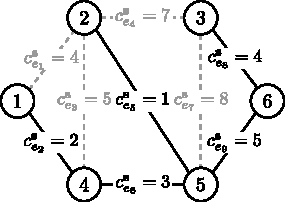
\includegraphics[width=\textwidth]{Chapter_II/INC-MST-example/a}
		\caption{}
		\label{fig:increxample:a}
	\end{subfigure}
	\hfill
	\begin{subfigure}[b]{0.3\textwidth}
		\includegraphics[width=\textwidth]{Chapter_II/INC-MST-example/b}
		\caption{}
		\label{fig:increxample:b}
	\end{subfigure}
	\hfill
	\begin{subfigure}[b]{0.3\textwidth}
		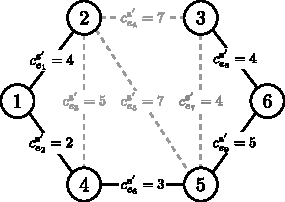
\includegraphics[width=\textwidth]{Chapter_II/INC-MST-example/c}
		\caption{}
		\label{fig:increxample:c}
	\end{subfigure}
	\hfill\null
	\caption{
		Różnice między rozwiązaniami problemów \textsc{Minimum Spanning Tree} i~\textsc{Incremental MST} z~parametrem $k = 1$.
		\textbf{(a)}~Optymalne rozwiązanie problemu minimalnego drzewa rozpinającego $T^{\ast}_{\textbf{s}}$ dla scenariusza $\textbf{s} = \left\{ 4, 2, 5, 7, 1, 3, 8, 4, 5 \right\}$ o~całkowitym koszcie rozwiązania $v_{\textsc{MST}} \left( T^{\ast}_{\textbf{s}}, \textbf{s} \right) = 15$.	
		\textbf{(b)}~Niedopuszczalne rozwiązanie $T^{\ast}_{\textbf{s}^{\prime}} = \left\{ e_{1}, e_{2}, e_{6}, e_{7}, e_{8} \right\}$ problemu \textsc{Incremental Minimum Spanning Tree}, będące jednocześnie optymalnym dla scenariusza $\textbf{s}^{\prime}$ w~problemie \textsc{MST} o~koszcie $v_{\textsc{MST}} \left( T^{\ast}_{\textbf{s}^{\prime}}, \textbf{s}^{\prime} \right) = 17$.
		\textbf{(c)}~Optymalne rozwiązanie problemu \textsc{Incremental MST} i~scenariusza $\textbf{s}^{\prime}$: $T^{\ast} = \left\{ e_{1}, e_{2}, e_{6}, e_{8}, e_{9} \right\}$ o~całkowitym koszcie $v^{\ast}_{\textbf{s}^{\prime}} = 18$.
	}
	\label{fig:increxample}
\end{figure}

Niestety wraz ze wzrostem grafu (oraz przede wszystkim parametru $k$) rozwiązanie to staje się nieefektywne --- jak mogliśmy zauważyć, opisany algorytm działa sekwencyjnie, co każdą iterację zmniejszając wartość funkcji $f \left( T^{i}, T \right)$, gdzie $T^{i}$ to rozwiązanie uzyskane podczas $i$-tej iteracji.
Ogólnie: $f \left( T^{i-1}, T \right) - 1 = f \left( T^{i}, T \right)$\footnote{
	W rozdziale \ref{ch:binaryIncMST} omówimy algorytm, który także działa iteracyjnie ze względu na wartość tej funkcji, lecz przedstawiona własność nie jest zachowana, co przekłada się na dużo lepsze otrzymywane czasy działania.
}.
Naszym zadaniem zatem jest konstrukcja takiego ciągu drzew rozpinających $T^{1}, \dots, T^{l}$, aby $f \left( T^{l}, T^{0} \right) = k$, gdzie $T^{0} = T$ i~jest początkowym rozwiązaniem problemu $\mathcal{P}$ dla pierwotnego scenariusza, zaś $l = f \left( T^{1}, T^{0} \right) - k + 1$ ($k = f \left( T^{l}, T^{0} \right) = f \left( T^{l-1}, T^{0} \right) - 1 = \dots =  f \left( T^{2}, T^{0} \right) - \left( l - 2 \right) = f \left( T^{1}, T^{0} \right) - \left( l - 1 \right) = k$ --- ogólnie $f \left( T^{l - i}, T^{0} \right) - i = k$).
Każde kolejne rozwiązanie powinno zatem składać się z~coraz to większej liczby krawędzi należących do $T^{0}$.
Aby to osiągnąć, dla każdej $i$-tej iteracji musielibyśmy rozpatrzyć wszystkie możliwe podziały drzewa $T^{i-1}$, powstałe w~wyniku usunięcia jednej z~krawędzi $e^{i-1} \in T^{i-1} \setminus T^{0}$ --- innymi słowy wszystkie takie pary drzew $\left( T^{i-1}_{1}, T^{i-1}_{2} \right)$, których łączna liczba krawędzi nie należących do drzewa $T^{0}$ jest o~$1$ mniejsza niż dla drzewa $T^{i-1}$. 
Takich par w~$i$--tej iteracji jest dokładnie $f \left( T^{1}, T^{0} \right) - k - \left( i - 1 \right)$ (iteracje numerujemy rozpoczynając od $i = 1$).
Dla każdej takiej pary musimy następnie znaleźć wszystkie krawędzie należące do zbioru $\mathcal{Q} \left( T^{i-1}, e^{i-1} \right) \cap T^{0}$, łączące ze sobą dane poddrzewa\footnote{
	O zbiorze krawędzi łączącym dwa poddrzewa rozpinające, które powstały w~wyniku cięcia oryginalnego drzewa, pisaliśmy w~poprzednim rozdziale (\ref{sec:mst}).
}, gdzie krawędź $e^{i-1} \in T^{i-1}$ jest krawędzią usuwaną z~$T^{i-1}$, nienależącą do $T^{0}$.
Na samym końcu musimy stworzyć nowe drzewo, do którego dołączymy krawędź $e^{\prime} \in \mathcal{Q} \left( T^{i-1}, e^{i-1} \right) \cap T^{0}$ o~najkorzystniejszym stosunku jej wagi do kosztu usuniętej krawędzi.
Formalnie: $T^{i} = \left( \left\{ e : e \in T^{i-1} \right\} \setminus e^{i-1} \right) \cup e^{\prime} \; : \; e^{\prime} = \min arg_{e^{\prime}} \frac{c_{e^{\prime}}}{c_{e^{i-1}}}$. 

Złożoność takiego rozwiązania to $O \left( \left| V \right| \cdot \left(l^{3} + \left| V \right| \right) \right)$, gdzie $l$ to liczba iteracji algorytmu (miara tego, jak daleko od dopuszczalności dla \textsc{Incremental MST} jest optymalne rozwiązanie dla problemu \textsc{MST}).
W~pierwszej iteracji liczba potencjalnych krawędzi do usunięcia wynosi $l - 1$ i~stopniowo maleje.
Dla każdej takiej krawędzi musimy zaś zdeterminować zbiór możliwych do dodania łuków.
Bez straty ogólności możemy założyć, że po uzyskaniu podziału drzewa $T^{i-1}$ na $\left( T^{i-1}_{1}, T^{i-1}_{2} \right)$, aby ustalić właściwy zbiór krawędzi, będziemy szukać odpowiednich łuków wychodzących z~wierzchołków, należących do drzewa o~mniejszej ich liczbie (będziemy analizować krawędzie wychodzące z~wierzchołków $v \in T^{i-1}_{1}$, jeśli $\left| \left\{ v_{i} : e_{ij} \in T^{i-1}_{1} \right\} \right| \leqslant \left| \left\{ v_{i} : e_{ij} \in T^{i-1}_{2} \right\} \right|$\footnote{
	Wyrażenie $\left| \left\{ v_{i} : e_{ij} \in T \right\} \right|$ oznacza po prostu liczbę wierzchołków, które łączą ze sobą krawędzie należące do drzewa $T$ --- jako że rozpatrujemy tylko grafy nieskierowane, $\left\{ v_{i} : e_{ij} \in T \right\} \equiv \left\{ v_{j} : e_{ij} \in T \right\}$ (kolejność wierzchołków w~zbiorach nie jest istotna).
}, bądź z~$v \in T^{i-1}_{2}$ w~przeciwnym przypadku).
Możemy założyć, że w~najgorszym z~możliwych przypadków wszystkie krawędzie, tworzące podział na poddrzewa $T^{i-1}_{1}$ oraz $T^{i-1}_{2}$, dzielą oryginalne drzewo $T^{i-1}$ na możliwie równe części --- każdorazowe ustalenie zbioru krawędzi $\mathcal{Q} \left( T^{i-1}, e^{i-1} \right)$ (a tym samym $\mathcal{Q} \left( T^{i-1}, e^{i-1} \right) \cap T^{0}$) zatem wymagać będzie od nas przeglądnięcia wszystkich krawędzi wychodzących z~$\frac{\left| V \right| - 1}{2} - \frac{i - j}{2}$ wierzchołków, gdzie $j$ to indeks krawędzi $e_{j}$, według której dokonujemy podziału.
Możemy także założyć, że w~pesymistycznym przypadku będziemy mieli do czynienia z~grafem pełnym, gdzie stopnień każdego wierzchołka $v \in V$ wynosi $d \left( v \right) = \left| V \right| - 1$.
Stąd otrzymujemy wzór na ogólną liczbę porównań wybranych par krawędzi $\left( e^{i-1}, e^{\prime} \right)$, gdzie $e^{i-1}$ jest krawędzią wychodzącą z~rozwiązania, zaś $e^{\prime}$ --- wchodzącą:

\begin{gather*}
	\sum_{\mathclap{i=1}}^{\mathclap{l-1}} \sum_{\mathclap{j=1}}^{\mathclap{i}} \left( \left| V \right| - 1 \right) \cdot \left( \frac{\left| V \right| - 1}{2} - \frac{i - j}{2} \right) = \frac{1}{12} \cdot \left( l - 3 \right) \cdot \left( \left| V \right| - 1 \right) \cdot \left( l^{2} - 3 \cdot l \cdot \left| V \right| + 2 \right) = \\ 
	= \frac{l^{3} \cdot \left( \left| V \right| - 1 \right)}{12} - \frac{l^{2} \cdot \left( \left| V \right|^{2} - 1 \right)}{4} + \frac{3 \cdot l \cdot \left| V \right|^{2}}{4} - \frac{7 \cdot l \cdot \left| V \right|}{12} - \frac{l}{6} - \frac{\left| V \right|}{2} + \frac{1}{2}\text{.}
\end{gather*}

Dodając do tego koszt odnalezienia potencjalnych krawędzi, które będziemy usuwać ($\left| V \right| - 1$ --- wystarczy raz przejść po wszystkich krawędziach drzewa $T^{0}$; z~każdą następną iteracją zbiór ten pomniejsza się o~ustaloną krawędź, więc nie musimy za każdym razem rozpoczynać analizy krawędzi drzewa od nowa), otrzymujemy --- wymieniony na samym początku --- stopień złożoności, który ilustruje wykres \ref{fig:incmst3D}.

\begin{figure}[!htbp]
	\renewcommand\figurename{Wykres}
	\null\hfill
	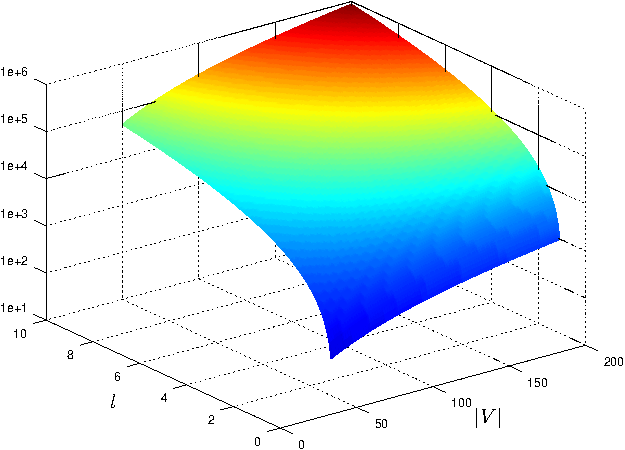
\includegraphics[width=0.65\textwidth]{Chapter_II/INC-MST-Other/incmst3DPlot_psfrag}
	\hfill\null
	\caption{
		Stopień złożoności naiwnego algorytmu rozwiązującego problem minimalnego drzewa rozpinającego w~wersji \textsc{Incremental} głównie zależy od liczby krawędzi, o~które optymalne rozwiązanie dla problemu \textsc{MST} różni się od dopuszczalnej liczby nowych krawędzi względem starego rozwiązania w~problemie \textsc{Incremental Minimum Spanning Tree}.
	}
	\label{fig:incmst3D}
\end{figure}

Najprostszym z~możliwych opisów tak zdefiniowanego problemu jest model przedstawiony w~\ref{mod:lpmodel1} dla nowego scenariusza $\textbf{s}^{\prime}$, gdzie $T_{0}$ oznacza nasze drzewo początkowe, $T^{\ast}$ --- optymalne rozwiązanie dla problemu \textsc{IMST}, gdzie $x_{e} = 1$ oznacza należenie do niego krawędzi $e \in E$. 

\newpage

\begin{subequations}
	\begin{alignat}{5}
	v^{\textsc{IMST}} \left( T^{\ast}, \textbf{s}^{\prime} \right) \; = \; & \text{min} & & \sum_{\mathclap{e \in E}} c^{\textbf{s}^{\prime}}_{e} \cdot x_{e}\text{,} \quad\quad &\\
	& & \quad & x_{e} = 1\text{,} & & \forall e \in T_{0}\text{,} & \quad\quad &\\
	& & & \sum_{\mathclap{e \in T^{\ast} \setminus T_{0}}} x_{e} \leqslant k \text{,} & & & \quad\quad &\\
	& & & \phantom{\sum} x_{e} \in \left\{ 0, 1 \right\}\text{,} && \forall e \in E\text{.} && \quad\quad &
	\end{alignat}\label{mod:lpmodel1}
\end{subequations}



\subsection{Zagadnienia oparte na problemie INCREMENTAL}



\subsubsection{Problem adwersarza}\label{sec:adv}


Przyjrzymy się teraz nieco bardziej rozbudowanemu problemowi, znanego jako \textbf{problem adwersarza} (ang. adversarial problem).
W~tym przypadku zamiast skupiać się na minimalizacji rozwiązania, naszym celem (celem adwersarza) jest maksymalizowanie jego wartości~\cite[$2$]{DBLP:journals/corr/NasrabadiO13}.
Osiągnąć cel możemy poprzez wybór takiego scenariusza, dla którego najlepsza wartość rozwiązania problemu \textsc{Incremental} będzie najgorsza:

\begin{equation}
	\max_{\mathclap{\textbf{s}^{\prime} \in S}} \min_{\mathclap{\textbf{y} \in X^{k}_{\textbf{x}}}} v \left( \textbf{y}, \textbf{s}^{\prime} \right)\text{.}
\end{equation}

Łatwo zauważyć, że oba te wybory --- adwersarza i~osoby wybierającej rozwiązanie dla problemu \textsc{Incremental} --- nie zależą od siebie, przez co problem sprowadza się do omawianego wcześniej, z~tą różnicą, że zamiast posiadania dwóch scenariuszy (gdzie na podstawie pierwszego wybieraliśmy rozwiązanie w~postaci wektora $\textbf{x}$), mamy ich większą liczbę i~adwersarz dla każdego z~nich musi policzyć wartość $\min_{\textbf{y} \in X^{k}_{\textbf{x}}} v \left( \textbf{y}, \textbf{s}^{\prime} \right)$, by móc wybrać najbardziej sprzyjający mu scenariusz (skutkujący zwróceniem jak największej wartości).
Problem można zatem bez trudu zrównoleglić (rozwiązywać jednocześnie klasyczny problem \textsc{IMST} dla wielu scenariuszy naraz), przez co nie da się o~nim napisać wiele więcej ponad to, co już napisaliśmy przy omawianiu wcześniejszego problemu.


\subsubsection{Odporny problem przyrostowy z~możliwością poprawy rozwiązania}


Kolejnym rozszerzeniem poprzednio omawianego problemu jest problem \textbf{odpornej optymalizacji przyrostowej} (ang. \textit{robust incremental optimization}~\cite[$2$]{DBLP:journals/corr/NasrabadiO13}).
W~odróżnieniu od problemów typu \textsc{Incremental} oraz problemu adwersarza, w~tym przypadku chcemy cofnąć się o~jeden krok w~procesie poszukiwania rozwiązania i~zminimalizować jego wartość, uwzględniając dodatkowo naszą pierwszą decyzję --- tą odnoszącą się do wektora $\textbf{x}$, będącą podstawą do rozwiązania problemu \textsc{Incremental}.
Jak możemy się domyślać, problem ten definiujemy w~następujący sposób:

\begin{equation}\label{eq:rimstdef}
	\min_{\mathclap{\textbf{x} \in X}} \left( v \left( \textbf{x}, \textbf{s} \right) + \max_{\mathclap{\textbf{s}^{\prime} \in S}} \min_{\mathclap{\textbf{y} \in X^{k}_{\textbf{x}}}} v \left( \textbf{y}, \textbf{s}^{\prime} \right) \right)\text{.}
\end{equation}

Niech początkowym scenariuszem, na podstawie którego wybierzemy wektor $\textbf{x}$, będzie $\textbf{s}_{0} = \left\{ 1, 1, 1, 1, 1, 1 \right\}$, zaś scenariuszami, spośród których będzie mógł wybierać adwersarz:

\begin{itemize}
	\item $\textbf{s}_{1} = \left\{ 4, 6, 1, 9, 3, 7 \right\}$ oraz
	\item $\textbf{s}_{2} = \left\{ 7, 3, 9, 1, 9, 4 \right\}$.
\end{itemize}

Oczywiście wybór scenariusza $\textbf{s}_{0}$ nie jest przypadkowy --- naszym celem jest pokazanie możliwej do osiągnięcia różnicy w~jakości rozwiązania dla dwóch różnych sposobów podejścia do zadanego problemu: klasycznego, polegającego na prostym wybraniu rozwiązania o~najmniejszym koszcie w~pierwszym kroku, z~pominięciem problemu adwersarza, tożsamym z~rozwiązaniem zagadnienia minimalnego drzewa rozpinającego dla pojedynczego scenariusza ($\min_{\textbf{x} \in X} v \left( \textbf{x}, \textbf{s} \right)$), oraz odpornego. 
Łatwo zauważyć, że w~przypadku tak dobranych scenariuszy (tak jak to pokazano na rysunkach od \ref{fig:robincrexample:a} do \ref{fig:robincrexample:f} oraz \ref{fig:robincrexampleopt}), na pozór nic nie znacząca decyzja o~pierwszym wyborze rozwiązania (jako że wszystkie koszty w~scenariuszu $\textbf{s}_{0}$ są sobie równe, dowolnie wybrane drzewo rozpinające charakteryzuje ten sam koszt --- będzie zatem wyborem optymalnym), w~przypadku pojawienia się odpowiednich zmian kosztów, może zaważyć na optymalności całego rozwiązania w~myśl \ref{eq:rimstdef}.
Dodatkowo niech parametr dla problemu \textsc{Incremental Minimum Spanning Tree} wynosi $k = 1$.
Przedstawiany na rysunkach \ref{fig:robincrexample:a}--\ref{fig:robincrexample:f}, \ref{fig:robincrexampleopt} graf jest na tyle nieduży, że z~powodzeniem możemy rozwiązać ten problem, wykorzystując do tego pełen przegląd wszystkich możliwych rozwiązań (ang. \textit{brute force}) --- dla każdego możliwego drzewa rozpinającego, reprezentowanego przez wektor $\textbf{x}$, możemy wyliczyć wartość $v \left( \textbf{x}, \textbf{s} \right) + \max_{\textbf{s}^{\prime} \in S} \min_{\textbf{y} \in X^{k}_{\textbf{x}}} v \left( \textbf{y}, \textbf{s}^{\prime} \right)$, rozwiązując po drodze $24$ egzemplarze problemu \textsc{Incremental Minimum Spanning Tree} (po dwa dla każdej z~$12$ instancji problemu \textsc{Adversarial Incremental Minimum Spanning Tree} --- $X = \left\{ \textbf{x}_{1}, \textbf{x}_{1}, \dots, \textbf{x}_{12} \right\}$).
Otrzymane wyniki zgromadzono w~tabeli \ref{tab:minmaxrobexample}, która reprezentuje wartości optymalnych rozwiązań poszczególnych składowych głównego problemu.
Tabela nie przedstawia natomiast wyników, uzyskanych dla problemu przedstawionego w~równaniu (\ref{eq:rimstdef}) --- możemy dostrzec, że dla tak specyficznie zdefiniowanego scenariusza $\textbf{s}_{0}$, suma kosztów wszystkich krawędzi w~dowolnie wybranym drzewie rozpinającym jest taka sama (wynosi $4$), więc wartości te możemy z~powodzeniem obliczyć sami (dodając tą wartość do przedstawionych wyników dla problemu adwersarza)\footnote{
	Ze względu na dość ogólne znaczenie, jakie ma zwrot odpornej optymalizacji przyrostowej, będziemy chcieli od niego uciec i~od tej pory odnosić się do naszego problemu, u~którego podstaw leży problem minimalnego drzewa rozpinającego w~wersji \textsc{Incremental}, jako do problemu \textsc{Recoverable Robust Incremental Minimum Spanning Tree} (dalej \textsc{RRIMST}), gdzie takie oznaczenie bezpośrednio wskazuje na podstawowy problem, z~jakim się będziemy zmagać.
	W~literaturze często możemy się dodatkowo spotkać z~inną jego nazwą: \textsc{k-Dist Recoverable Robust Spanning Tree}~\cite{Kasperski2014}.
}.

\begin{table}[!htbp]
	\caption{
		Tabela przedstawiająca wszystkie, możliwe do skonstruowania dla grafu prezentowanego na rysunkach od \ref{fig:robincrexample:a} do \ref{fig:robincrexample:f} oraz \ref{fig:robincrexampleopt}, drzewa rozpinające, reprezentowane przez wektory od $\textbf{x}_{1}$ do $\textbf{x}_{12}$, wartości optymalnych rozwiązań problemów \textsc{Incremental Minimum Spanning Tree} dla wszystkich scenariuszy adwersarza ($\textbf{s}_{1}$ oraz $\textbf{s}_{2}$) z~uwzględnieniem parametru $k = 1$ oraz (w ostatniej kolumnie) wartość optymalnego rozwiązania problemu adwersarza dla zbioru jego scenariuszy oraz danego wektora początkowego $\textbf{x}$.
		Rozwiązania, reprezentowane przez wektory od $\textbf{x}_{1}$ do $\textbf{x}_{12}$, są posortowane według rosnącej wartości dla odpowiadającego im rozwiązania problemu \textsc{Adversarial Incremental Minimum Spanning Tree}.
	}
	\label{tab:minmaxrobexample}
	\begin{tabular}{cccccccccc}
		\cline{8-10}
		\multicolumn{2}{l}{}       &         &         &         &         &         & \multicolumn{3}{c}{Scenariusze}                                                                                                                                                                                              \\
		$X$              & $e_{1}$ & $e_{2}$ & $e_{3}$ & $e_{4}$ & $e_{5}$ & $e_{6}$ & 	\footnotesize$v^{\textsc{IMST}}_{\textbf{s}_{1}} = \min_{\textbf{y} \in X^{k}_{\textbf{x}}} v \left( \textbf{y}, \textbf{s}_{1} \right) $ &\footnotesize $v^{\textsc{IMST}}_{\textbf{s}_{2}} = \min_{\textbf{y} \in X^{k}_{\textbf{x}}} v \left( \textbf{y}, \textbf{s}_{2} \right)$ &\footnotesize $\max \left\{ v^{\textsc{IMST}}_{\textbf{s}_{1}}, v^{\textsc{IMST}}_{\textbf{s}_{2}} \right\} $ \\\normalsize
		$\textbf{x}_{1}$	&	$1$	&	$1$	&	$0$	&	$1$	&	$1$	&	$0$	&	$14$	&	$15$	&	$15$	\\
		$\textbf{x}_{2}$	&	$1$	&	$0$	&	$0$	&	$1$	&	$1$	&	$1$	&	$15$	&	$15$	&	$15$	\\
		$\textbf{x}_{3}$	&	$0$	&	$1$	&	$0$	&	$1$	&	$1$	&	$1$	&	$17$	&	$15$	&	$17$	\\
		$\textbf{x}_{4}$	&	$0$	&	$1$	&	$1$	&	$0$	&	$1$	&	$1$	&	$14$	&	$17$	&	$17$	\\
		$\textbf{x}_{5}$	&	$1$	&	$0$	&	$1$	&	$1$	&	$0$	&	$1$	&	$15$	&	$15$	&	$15$	\\
		$\textbf{x}_{6}$	&	$0$	&	$1$	&	$1$	&	$1$	&	$0$	&	$1$	&	$17$	&	$15$	&	$17$	\\
		$\textbf{x}_{7}$	&	$1$	&	$1$	&	$1$	&	$0$	&	$0$	&	$1$	&	$14$	&	$15$	&	$15$	\\
		$\textbf{x}_{8}$	&	$1$	&	$0$	&	$1$	&	$0$	&	$1$	&	$1$	&	$14$	&	$21$	&	$21$	\\
		$\textbf{x}_{9}$	&	$1$	&	$0$	&	$1$	&	$1$	&	$1$	&	$0$	&	$14$	&	$20$	&	$20$	\\
		$\textbf{x}_{10}$	&	$0$	&	$1$	&	$1$	&	$1$	&	$1$	&	$0$	&	$14$	&	$17$	&	$17$	\\
		$\textbf{x}_{11}$	&	$1$	&	$1$	&	$1$	&	$0$	&	$1$	&	$0$	&	$14$	&	$20$	&	$20$	\\
		$\textbf{x}_{12}$	&	$1$	&	$1$	&	$0$	&	$1$	&	$0$	&	$1$	&	$18$	&	$15$	&	$18$	\\
		\hline
	\end{tabular}
\end{table}

\begin{figure}[!htbp]
	\null\hfill
	\begin{subfigure}[b]{0.3\textwidth}
		\includegraphics[width=\textwidth]{Chapter_II/ROB-INC-MST-example/a1}
		\caption{}
		\label{fig:robincrexample:a}
	\end{subfigure}
	\hfill
	\begin{subfigure}[b]{0.3\textwidth}
		\includegraphics[width=\textwidth]{Chapter_II/ROB-INC-MST-example/b1}
		\caption{}
		\label{fig:robincrexample:b}
	\end{subfigure}
	\hfill
	\begin{subfigure}[b]{0.3\textwidth}
		\includegraphics[width=\textwidth]{Chapter_II/ROB-INC-MST-example/c1}
		\caption{}
		\label{fig:robincrexample:c}
	\end{subfigure}
	\hfill\null
	\caption{
		Sytuacja dla problemu \textsc{Recoverable Robust Incremental Minimum Spanning Tree} dla wybranego rozwiązania $T = T_{\textbf{x}_{5}} = \left\{ e_{1}, e_{3}, e_{4}, e_{6} \right\}$, gdzie dwa ostatnie rysunki prezentują drzewa, z~których rozwiązanie wybierać będzie adwersarz.
		\textbf{(a)}~Drzewo rozpinające wybrane przez podejmującego decyzję (nie przez adwersarza), reprezentowane przez wektor $\textbf{x}_{5} = \left[ 1, 0, 1, 1, 0, 1 \right]$ (patrz: tabela \ref{tab:minmaxrobexample}) o~sumie kosztów wybranych krawędzi $v \left( T, \textbf{s}_{0} \right) = 4$.
		\textbf{(b)}~Minimalne drzewo rozpinające $T^{\textsc{IMST}}_{\textbf{s}_{1}}$ o~najmniejszym koszcie dla problemu typu \textsc{Incremental} z~parametrem $k = 1$ oraz drzewem początkowym $T$.
		Krawędzią, która weszła do rozwiązania nowego drzewa, jest $e_{5}$ ($T^{\textsc{IMST}}_{\textbf{s}_{1}} \setminus T = \left\{ e_{5} \right\}$), zaś usuniętą --- $e_{4}$.
		Koszt rozwiązania wynosi $15$.
		\textbf{(c)}~Rozwiązanie problemu \textsc{Incremental Minimum Spanning Tree} dla drugiego scenariusza ($\textbf{s}_{2}$) i~tego samego początkowego drzewa rozpinającego $T$.
		Liczba krawędzi nie należących do drzewa $T$, jednocześnie zawierających się w~nowym rozwiązaniu $T^{\textsc{IMST}}_{\textbf{s}_{2}}$, wynosi $1$.
		W~obu przypadkach koszt optymalnych rozwiązań danego problemu jest taki sam ($v \left(  T^{\textsc{IMST}}_{\textbf{s}_{1}}, \textbf{s}_{1} \right) = v \left(  T^{\textsc{IMST}}_{\textbf{s}_{2}}, \textbf{s}_{2} \right) = 15$), toteż wybór scenariusza ($\textbf{s}_{1}$ lub $\textbf{s}_{2}$), który zostanie podjęty przez adwersarza, nie ma żadnego znaczenia (dla rozwiązania reprezentowanego przez $\textbf{x}_{5}$).
	}
\end{figure}

\begin{figure}[!htbp]
	\null\hfill
	\ContinuedFloat
	\begin{subfigure}[b]{0.3\textwidth}
		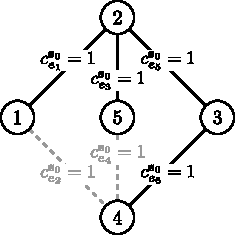
\includegraphics[width=\textwidth]{Chapter_II/ROB-INC-MST-example/a2}
		\caption{}
		\label{fig:robincrexample:d}
	\end{subfigure}
	\hfill
	\begin{subfigure}[b]{0.3\textwidth}
		\includegraphics[width=\textwidth]{Chapter_II/ROB-INC-MST-example/b2}
		\caption{}
		\label{fig:robincrexample:e}
	\end{subfigure}
	\hfill
	\begin{subfigure}[b]{0.3\textwidth}
		\includegraphics[width=\textwidth]{Chapter_II/ROB-INC-MST-example/c2}
		\caption{}
		\label{fig:robincrexample:f}
	\end{subfigure}
	\hfill\null
	\caption{
		Wybrane drzewo rozpinające $T_{\textbf{x}_{8}}$ (patrz: tabela \ref{tab:minmaxrobexample}) dla problemu \textsc{Recoverable Robust Incremental Minimum Spanning Tree} wraz z~dwoma drzewami, będącymi optymalnymi rozwiązaniami problemu \textsc{Incremental Minimum Spanning Tree} odpowiednio dla scenariuszy $\textbf{s}_{1}$ oraz $\textbf{s}_{2}$.
		\textbf{(d)}~Wybrane rozwiązanie, reprezentowane przez wektor $\textbf{x}_{8} = \left[ 1, 0, 1, 0, 1, 1 \right]$, o~koszcie $4$.
		\textbf{(e)}~Optymalne rozwiązanie problemu minimalnego drzewa rozpinającego w~wersji \textsc{Incremental} dla scenariusza $\textbf{s}_{1}$ (początkowego $\textbf{s}_{0}$) o~wartości rozwiązania równej $14$.
		\textbf{(f)}~Minimalne drzewo rozpinające, które jest optymalnym rozwiązaniem dla tego samego problemu, dla scenariusza $\textbf{s}_{2}$.
		Jako że koszt tego rozwiązania jest największy spośród wszystkich rozwiązań problemu \textsc{IMST} dla scenariuszy adwersarza (koszt tego rozwiązania wynosi $21$), zostanie ono przez niego wybrane.
		Poprzednie rozwiązanie (o koszcie $14$) zostanie odrzucone jako nieopłacalne.
	}
	\label{fig:robincrexample}
\end{figure}

\begin{figure}[!h]
	\null\hfill
	\begin{subfigure}[b]{0.3\textwidth}
		\includegraphics[width=\textwidth]{Chapter_II/ROB-INC-MST-example/d1}
		\caption{}
		\label{fig:robincrexampleopt:a}
	\end{subfigure}
	\hfill
	\begin{subfigure}[b]{0.3\textwidth}
		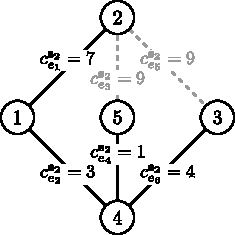
\includegraphics[width=\textwidth]{Chapter_II/ROB-INC-MST-example/d2}
		\caption{}
		\label{fig:robincrexampleopt:b}
	\end{subfigure}
	\hfill\null
	\caption{
		Optymalne rozwiązania problemów \textsc{Incremental Minimum Spanning Tree} dla podwyższonej wartości parametru $k = 2$, która dla prezentowanego grafu jest wystarczająca, aby zwracane rozwiązania dla poszczególnych scenariuszy były takie same jak dla klasycznego problemu minimalnego drzewa rozpinającego.
		\textbf{(a)}~Minimalne drzewo rozpinające dla scenariusza $\textbf{s}_{1} = \left[ 4, 6, 1, 9, 3, 7 \right]$.
		\textbf{(b)}~Optymalne rozwiązanie problemu minimalnego drzewa rozpinającego w~wersji \textsc{Incremental} dla scenariusza $\textbf{s}_{2}$.
	}
	\label{fig:robincrexampleopt}
\end{figure}

Widzimy zatem jak bardzo skomplikowanym i~trudnym obliczeniowo procesem jest generowanie rozwiązań dla problemu \textsc{Recoverable Robust Incremental Minimum Spanning Tree} i~jak ciężko musieliśmy pracować, aby dojść do tego punktu (po drodze poznaliśmy dwa inne problemy, które są tylko jego częścią).
Poziom złożoności opisanego przez nas problemu dodatkowo potęguje fakt, że przedstawiony przez nas przykład tyczył się grafu o~bardzo niewielkich rozmiarach --- liczył on sobie zaledwie $6$ krawędzi i~$5$ wierzchołków.
Jego konstrukcja z~kolei w~bardzo znaczący sposób ograniczyła liczbę możliwych rozwiązań (liczebność zbioru $X$), my zaś jeszcze bardziej uprościliśmy problem, wybierając do problemu adwersarza najmniejszą liczbę scenariuszy, jaka ma jeszcze dla tego problemu sens ($\textbf{s}_{1}$, $\textbf{s}_{2}$).
W ogólnym przypadku nie możemy mieć nadziei, że takie podejście do problemu (rozwiązanie siłowe) będzie możliwe.




\section{Podsumowanie rozdziału}




Widzimy, że sposobów podejścia do problemów optymalizacyjnych jest bardzo dużo, zaś te przez nas przedstawione stanowią już dużo bardziej zaawansowane spojrzenie na ten problem, niż pokazaliśmy w~poprzednim rozdziale, omawiając podstawowe pojęcia związanie z~problemem minimalnego drzewa rozpinającego.
Wraz z~omawianiem kolejnych zagadnień w~tym rozdziale mogliśmy zauważyć naszą potrzebę konstrukcji takich rozwiązań, które nie tylko pozwalać nam będą wybierać najlepsze dla nas rozwiązania, gdy zawczasu przewidzimy wszystkie możliwe sytuacje (im większy zbiór zdarzeń zostanie przez nas uwzględniony, tym bardziej ogólne rozwiązanie najprawdopodobniej wybierzemy), ale i~na bieżąco będą reagować na zaistniałe sytuacje (co pozwala na wybór znacznie lepszych rozwiązań, uwzględniających tylko najbliższą przyszłość).
Dodatkowo chcieliśmy, aby tak konstruowane rozwiązania łatwo poddawały się zmianom --- aby wybór jednego (optymalnego w~czasie jego wyboru) nie powodował konieczności jego całkowitej rekonstrukcji w~przypadku zajścia przewidzianego przez nas scenariusza.
W~związku z~tym podaliśmy formułę, która wybiera dla nas takie rozwiązania, które nie tylko łatwo modyfikować (poprawiać), ale i~takie, które zapewniają najlepsze rezultaty w~najbliższej, przewidzianej przez nas, przyszłości.
Niestety wraz z~rosnącymi oczekiwaniami oczywiście rósł poziom skomplikowania opisywanych problemów i~dla ostatniego z~nich (\textsc{Recoverable Robust Incremental Minimum Spanning Tree} z~dyskretnym zbiorem scenariuszy $S$) zwyczajnie nie jesteśmy już w~stanie podać wielomianowego algorytmu, który radziłby sobie z~danym problemem (w przypadku dwóch pozostałych --- \textsc{Adversarial Incremental Minimum Spanning Tree} oraz \textsc{Incremental Minimum Spanning Tree} --- podamy je w~następnych rozdziałach).
W~związku z~tym, w~rozdziale \ref{ch:localSearch} przedstawimy inną metodę podejścia do danego problemu (heurystyczną).
Dodatkowo warto w~tym miejscu podkreślić, że wszystkie do tej pory omówione przypadki problemów koncentrowały się na znanej, ograniczonej przez daną stałą, liczbie scenariuszy (z góry ustalonym, dyskretnym ich zbiorze $S$), co zdecydowanie upraszcza sposób patrzenia się na te problemy --- analizę przez nas omawianych przypadków (tyle że dla nieograniczonej liczby scenariuszy, gdzie ich liczba jest częścią danych wejściowych dla problemu) możemy znaleźć w~\cite{DBLP:journals/ipl/KasperskiZ09}.
Następnym rozdziałem odejdziemy nieco od omawianych jak dotąd problemów --- wyjaśnimy znaczenie modelu (równania \ref{mod:lpmodel1}), przedstawiając podstawowe pojęcia z~nieco innego obszaru algorytmiki --- programowania \textsc{LP}, \textsc{MIP} oraz \text{IP}.